\documentclass[18pt,xcolor=table]{beamer}
\usepackage{etex}
\reserveinserts{28}
\usepackage{amsmath, amssymb, amsthm, mathtools}
\usepackage{graphicx}
\usepackage{cancel}
\usepackage{color}
\usepackage{caption}
\usepackage{subcaption}
%\usepackage{subfigure}
\usepackage{pgf,tikz}
\usetikzlibrary{arrows}

\captionsetup{compatibility=false}

\newcommand{\bs}[1]{\boldsymbol{#1}}
\newcommand{\norm}[1]{\left\| #1 \right\|}
\newcommand{\snorm}[1]{\left| #1 \right|}
\newcommand{\LRp}[1]{\left( #1 \right)}
\newcommand{\LRs}[1]{\left[ #1 \right]}
\newcommand{\LRc}[1]{\left\{ #1 \right\}}
\newcommand{\LRa}[1]{\left\langle #1 \right\rangle}
\newcommand{\LRb}[1]{\left| #1 \right|}
\newcommand{\Grad}{\ensuremath{\nabla}}
\newcommand{\Gradxt}{\ensuremath{\nabla_{xt}}}
\newcommand{\Div}{\ensuremath{\nabla\cdot}}
\newcommand{\Divxt}{\ensuremath{\nabla_{xt}\cdot}}
\newcommand{\Curl}{\ensuremath{\nabla\times}}
\newcommand{\bfH}{\mbox{\boldmath $H$}}
\newcommand{\bfsigma}{\boldsymbol\sigma}
\newcommand{\bfvarsigma}{\boldsymbol\varsigma}
\newcommand{\bftau}{\boldsymbol\tau}
\newcommand{\bfbeta}{\boldsymbol\beta}
\newcommand{\bflambda}{\boldsymbol\lambda}
\newcommand{\bfpsi}{\boldsymbol\psi}
\newcommand{\bfu}{\boldsymbol u}
\newcommand{\bfv}{\boldsymbol v}
\newcommand{\bfV}{\boldsymbol V}
\newcommand{\bfZ}{\boldsymbol Z}
\newcommand{\bfz}{\boldsymbol z}
\newcommand{\bfW}{\boldsymbol W}
\newcommand{\bfw}{\boldsymbol w}
\newcommand{\bfm}{\boldsymbol m}
\newcommand{\bfM}{\boldsymbol M}
\newcommand{\bbM}{\mathbb{M}}
\newcommand{\bfq}{\boldsymbol q}
\newcommand{\bfU}{\boldsymbol U}
\newcommand{\bfS}{\boldsymbol S}
\newcommand{\bbS}{\mathbb{S}}
\newcommand{\bbD}{\mathbb{D}}
\newcommand{\bfK}{\boldsymbol K}
\newcommand{\bbK}{\mathbb{K}}
\newcommand{\bfn}{\boldsymbol n}
\newcommand{\bff}{\boldsymbol f}
\newcommand{\bfF}{\boldsymbol F}
\newcommand{\bbF}{\mathbb{F}}
\newcommand{\bfg}{\boldsymbol g}
\newcommand{\bfG}{\boldsymbol G}
\newcommand{\bfC}{\boldsymbol C}
\newcommand{\bft}{\boldsymbol t}
\newcommand{\bfT}{\boldsymbol T}
\newcommand{\bfI}{\boldsymbol I}
\newcommand{\bbI}{\mathbb{I}}
\newcommand{\bfx}{\boldsymbol x}
\newcommand{\uh}{\widehat{u}}
\newcommand{\fnh}{\widehat{f}_n}
\newcommand{\LQ}{L^2\LRp{Q}}
\newcommand{\LK}{L^2\LRp{K}}
\newcommand{\LVecK}{\mathbf{L}^2\LRp{K}}
\newcommand{\LVecQ}{\mathbf{L}^2\LRp{Q}}
\newcommand{\HdivK}{\bfH(\text{div},K)}
\newcommand{\HdivOmega}{\bfH(\text{div},\Omega)}
% \newcommand{\HdivOmegaLT}{\bfH(\text{div},\Omega)\times L^2([0,T])}
\newcommand{\HdivQ}{\bfH(\text{div}_{xt},Q)}
\newcommand{\HOneK}{H^{1}(K)}
\newcommand{\HOneVecK}{\bfH^{1}(K)}
\newcommand{\HOneQ}{H^{1}(Q)}
\newcommand{\HOneOmegah}{H^{-1}(\Omega_h)}
\newcommand{\HdivOmegah}{\bfH(\text{div},\Omega_h)}
\newcommand{\vdeltau}{v_{\delta\bs u_h}}
\newcommand{\taudeltau}{\bftau_{\delta\bs u_h}}
\newcommand{\ip}[1]{\left\langle #1 \right\rangle}
\newcommand{\pd}[2]{\frac{\partial#1}{\partial#2}}
\newcommand{\pt}[1]{\frac{\partial#1}{\partial t}}
\newcommand{\ppd}[2]{\frac{\partial^2#1}{\partial#2^2}}
\newcommand{\pdd}[3]{\frac{\partial^2#1}{\partial#2\partial#3}}
\newcommand{\der}[2]{\frac{\mathrm{d}#1}{\mathrm{d}#2}}
\newcommand{\Oh}{\Omega_h}
\newcommand{\jump}[1] {\ensuremath{\LRs{\![#1]\!}}}
\newcommand{\Gh}{\Gamma_h}
\newcommand{\mcU}{\mathcal{U}}
\newcommand{\mcUh}{\hat{\mathcal{U}}}
\newcommand{\LOmega}{L^2\LRp{\Omega_h}}

\newcommand{\eqnref}[1]{\eqref{eq:#1}}

\DeclareMathOperator*{\argmin}{arg\,min}
\DeclareMathOperator*{\trace}{tr}

\def\arrtwo#1#2#3#4{\left[
\begin{array}{cc}
#1\; & #2\\
#3\; & #4\\
\end{array}
\right]}
\def\arrthree#1#2#3#4#5#6#7#8#9{\left[
\begin{array}{ccc}
#1\; & #2\; & #3\\
#4\; & #5\; & #6\\
#7\; & #8\; & #9\\
\end{array}
\right]}
\def\arrthreeone#1#2#3{\left[
\begin{array}{ccc}
#1\; & #2\; & #3\\
\end{array}
\right]}
\def\vecttwo#1#2{\left(
\begin{array}{c}
#1\\
#2\\
\end{array}
\right)}
\def\svecttwo#1#2{\left[
\begin{array}{c}
#1\\
#2\\
\end{array}
\right]}
\def\vectthree#1#2#3{\left(
\begin{array}{c}
#1\\
#2\\
#3\\
\end{array}
\right)}
\def\svectthree#1#2#3{\left[
\begin{array}{c}
#1\\
#2\\
#3\\
\end{array}
\right]}

\renewcommand{\arraystretch}{1.2}

\def\etal{{\it et al.~}}

\graphicspath{{../PD13/figs/}{../Proposal/figs/}{../Figures/}}

\usepackage{bbm}
\usepackage{textpos}
\usepackage{pgf,tikz}
\usepackage{pgfplots}
\usepackage[space]{grffile}
\usepackage{graphicx}
\usepackage{forloop}
% \usepackage[aps,prb,citeautoscript]{revtex4-1}
% \usepackage[super]{natbib}
\usepackage[backend=bibtex]{biblatex}
\usepackage{animate}
\usepackage{listings}
\usepackage{bbding}
\usepackage{comment}
\bibliography{../Papers}

\newcounter{nn}

\AtBeginSection[]
{
  \begin{frame}
    \frametitle{Table of Contents}
    \framesubtitle{\hspace{1ex}}
    \tableofcontents[currentsection,currentsubsection]
  \end{frame}
}
\AtBeginSubsection[] {
  \begin{frame}
    \frametitle{Table of Contents}
    \framesubtitle{\hspace{1ex}}
    \tableofcontents[currentsection,currentsubsection]
  \end{frame}
}

\definecolor{utorange}{RGB}{203,96,21}
\definecolor{utblack}{RGB}{99,102,106}
\definecolor{utbrown}{RGB}{110,98,89}
\definecolor{utsecbrown}{RGB}{217,200,158}
\definecolor{utsecgreen}{RGB}{208,222,187}
\definecolor{utsecblue}{RGB}{127,169,174}

\mode<presentation>
{
  % \usetheme{Pittsburgh}
  \usetheme{Boadilla}
  \usefonttheme[onlymath]{serif}

  \setbeamercovered{invisible}
  \setbeamertemplate{navigation symbols}{}

  % Color Theme
    \setbeamercolor{normal text}{bg=white,fg=utblack}
  \setbeamercolor{structure}{fg=utorange}

  \setbeamercolor{alerted text}{fg=red!85!black}

  \setbeamercolor{item projected}{use=item,fg=black,bg=item.fg!35}

  \setbeamercolor*{palette primary}{use=structure,fg=white, bg=utorange}
  \setbeamercolor*{palette secondary}{use=structure,bg=utsecbrown}
  \setbeamercolor*{palette tertiary}{use=structure,bg=utsecgreen}
  \setbeamercolor*{palette quaternary}{use=structure,fg=structure.fg,bg=utsecblue}

  % \setbeamercolor*{frametitle}{use=structure,fg=utorange, bg=utsecbrown}
  \setbeamercolor*{framesubtitle}{fg=utbrown}

  \setbeamercolor*{block title}{parent=structure,fg=black,bg=utsecgreen}
  \setbeamercolor*{block body}{fg=black,bg=utblack!10}
  \setbeamercolor*{block title alerted}{parent=alerted text,bg=black!15}
  \setbeamercolor*{block title example}{parent=example text,bg=black!15}

  \setbeamerfont{framesubtitle}{size=\small}
}

% \usepackage[orientation=landscape,size=custom,width=16,height=9.75,scale=0.5,debug]{beamerposter}
% \usepackage[orientation=landscape,size=custom,width=16,height=9,scale=0.5,debug]{beamerposter}


\makeatletter
\setbeamertemplate{footline}
{
  \leavevmode%
    \hbox{%
      \begin{beamercolorbox}[wd=.333333\paperwidth,ht=2.25ex,dp=1ex,center]{author in head/foot}%
        \usebeamerfont{author in head/foot}\insertshortauthor%~~\beamer@ifempty{\insertshortinstitute}{}{(\insertshortinstitute)}
      \end{beamercolorbox}%
        \begin{beamercolorbox}[wd=.333333\paperwidth,ht=2.25ex,dp=1ex,center]{title in head/foot}%
        \usebeamerfont{title in head/foot}\insertshorttitle
        \end{beamercolorbox}%
        \begin{beamercolorbox}[wd=.333333\paperwidth,ht=2.25ex,dp=1ex,right]{date in head/foot}%
        \usebeamerfont{date in head/foot}\insertshortdate{}\hspace*{2em}
        \insertframenumber{} / \inserttotalframenumber\hspace*{2ex}
      \end{beamercolorbox}}%
        \vskip0pt%
}
\makeatother

\usepackage{kerkis}
\usepackage[T1]{fontenc}
\usepackage[protrusion=true,expansion=true]{microtype}
\usepackage{amsmath}


\renewcommand*{\thefootnote}{\fnsymbol{footnote}}

\let\oldfootnotesize\footnotesize
\renewcommand*{\footnotesize}{\oldfootnotesize\tiny}


\pgfdeclareimage[height=1.2cm]{utbig}{logos/UTWordmark}
\pgfdeclareimage[height=0.6cm]{ut}{logos/UTWordmark}
% \pgfdeclareimage[height=10.0cm]{utbig}{logos/ICES-wordmark-teal.pdf}
% \pgfdeclareimage[height=0.6cm]{ut}{logos/ICES-wordmark-teal.pdf}
% \pgfdeclareimage[height=1.5cm]{iceslogo}{logos/ICES-wordmark-teal.png}
% \pgfdeclareimage[height=1.0cm]{scsmall}{logos/SC12}

% \title[Space-Time DPG for Transient CFD]{Space-Time Discontinuous Petrov-Galerkin Finite Elements\\ for Transient Computational Fluid Dynamics}
\title[Automated Scientific Computing with DPG]{Automating Scientific Computing with Discontinuous Petrov-Galerkin Finite Elements}
% \subtitle{If you have one}
\author[Truman E. Ellis]{ \underline{Truman~Ellis} \\
{\oldfootnotesize \smallskip Collaborators: Leszek Demkowicz, Robert Moser, \\Nate Roberts (Argonne), Jesse Chan (Rice)}
}

\begin{comment}
The discontinuous Petrov-Galerkin method is a novel finite element framework with exceptional stability and adaptivity properties.
The DPG framework can be used to derive stable discretizations of any well-posed variational formulation 
and has been successfully applied to problems such as heat conduction, time-harmonic Helmholtz, 
Maxwell's equations, linear elasticity and plate problems, Stokes flow, and both incompressible and compressible Navier-Stokes.
In contrast to many other numerical methods, DPG does not suffer from a pre-asymptotic regime (unstable behavior on coarse meshes).
This means that a simulation can be initiated at the coarsest scale possible while automatic adaptivity resolves solution features 
based on a robust, built-in measure of residual error.
DPG is intensely locally compute intensive with significant embarrassingly parallel computations done both pre- and post-global solve.
We present preliminary work on a space-time DPG formulation that enables automatic local time stepping and a kind of parallel-in-time integration.
We also present the Camellia library, which is built on top of Trilinos and 
supports rapid specification of DPG problems while maintaining computational efficiency and scalability.
% Parallel to our efforts 
% In our efforts to create an automatic computational methodology, we have also 

% In addition to the automaticity of coarse-mesh stability and adaptivity, DPG is very locally compute intensive, making it ideal for HPC systems.

% Initial mesh design is a time consuming and expensive part of CFD simulations as a domain expert has to manually design the 
% mesh to achieve near resolution in all parts of the domain lest the numerical method become unstable.
% DPG in contrast does not have a pre-asymptotic regime, allowing simulations to start on the coarsest mesh that can adequately represent the domain geometry.
% \emph{A posteriori} error estimation and adaptivity can also be done very naturally as DPG comes with an error representation function 
% that indicates error in the energy norm.

% Automatic adaptivity and pre-asymptotic stability produce a powerful synergy when combined with high performance computing.
% Human intervention to correct or adapt a failed massively parallel simulation can be a costly endeavor, prompting the desire for a
% numerical technology that will automatically adapt to changing physical dynamics while avoiding ``crashing'' due to under-resolved meshes.
% DPG is very compute intensive compared to the associated communication and memory costs.
% Most of the work is spent in embarrassingly parallel local solves for the optimal test functions and local stiffness matrix assembly.
% Locally computed \emph{optimal test functions} ensure stability on convection dominated flows as well as resolved viscous flow.
% The division of degrees of freedom into internal vs skeleton unknowns produces a global system which can be statically condensed into 
% a solve purely in terms of the skeleton degrees of freedom.
% In addition to significantly cutting down on the size of the global solve, 
% this produces a embarrassingly parallel post-processing solve for the internal degrees of freedom.

% We recently began exploring the extension of these attractive DPG properties to space-time domains, allowing us to automate and localize temporal adaptivity
% in the same way that we already do with spatial adaptivity. Preliminary results have been generated with Camellia\cite{Roberts2011} for spatially 1D flows,
% and a rewrite of Camellia for higher dimensions is currently in progress.
\end{comment}

% \institute{Institute for Computational Engineering \& Sciences\\ \mbox{}  \\  \pgfuseimage{utbig} }
\institute{
\pgfuseimage{utbig}
\\ \vspace{2ex}

\includegraphics[trim=3.0in 7.2in 1.5in 4.0in,width=0.3\linewidth]{logos/ICES-wordmark-teal.pdf}
}
\date[Sandia National Laboratory]%{\pgfuseimage{iceslogo} }

\begin{document}
\def\thefootnote{\arabic{footnote}}

\tikzstyle{block} = [rectangle, draw, rounded corners, shade, top color=white, text width=5em,
  bottom color=blue!50!black!20, draw=blue!40!black!60, very thick, text centered, minimum height=4em]
  \tikzstyle{line} = [draw, -latex']
  \tikzstyle{cloud} = [draw, ellipse,top color=white, bottom color=red!20, node distance=2cm, minimum height=2em]


  \beamertemplateballitem
  %\beamertemplatetransparentcoveredhigh

  \frame{\titlepage}

  \addtobeamertemplate{frametitle}{}{%
      \begin{textblock*}{100mm}(0.87\textwidth,-0.75cm)
    \pgfuseimage{ut}
    \end{textblock*}
  }

%   /$$      /$$             /$$     /$$                        /$$     /$$                    
%  | $$$    /$$$            | $$    |__/                       | $$    |__/                    
%  | $$$$  /$$$$  /$$$$$$  /$$$$$$   /$$ /$$    /$$  /$$$$$$  /$$$$$$   /$$  /$$$$$$  /$$$$$$$ 
%  | $$ $$/$$ $$ /$$__  $$|_  $$_/  | $$|  $$  /$$/ |____  $$|_  $$_/  | $$ /$$__  $$| $$__  $$
%  | $$  $$$| $$| $$  \ $$  | $$    | $$ \  $$/$$/   /$$$$$$$  | $$    | $$| $$  \ $$| $$  \ $$
%  | $$\  $ | $$| $$  | $$  | $$ /$$| $$  \  $$$/   /$$__  $$  | $$ /$$| $$| $$  | $$| $$  | $$
%  | $$ \/  | $$|  $$$$$$/  |  $$$$/| $$   \  $/   |  $$$$$$$  |  $$$$/| $$|  $$$$$$/| $$  | $$
%  |__/     |__/ \______/    \___/  |__/    \_/     \_______/   \___/  |__/ \______/ |__/  |__/
%                                                                                              
%                                                                                              
\section{Motivation: Automating Scientific Computing}
% ------------------------------------------------------------
\begin{frame}[t]
\frametitle{Navier-Stokes Equations}
\framesubtitle{Numerical Challenges}
\begin{columns}[c]
\begin{column}{.6\textwidth}
Robust simulation of unsteady fluid dynamics remains a challenging issue.
\vspace{2ex}

\begin{itemize}
\item{} Resolving solution features (sharp, localized viscous-scale phenomena)
\begin{itemize}
\item{} Shocks
\item{} Boundary layers - resolution needed for drag/load
\item{} Turbulence (non-localized)
\end{itemize}
% \item{} Nonlinear convergence and uniqueness of solutions
\item{} Stability of numerical schemes
\begin{itemize}
\item{} Coarse/adaptive grids
\item{} Higher order
\end{itemize}
\end{itemize}
\end{column}
\begin{column}{.4\textwidth}
\vspace{-3ex}
\begin{figure}
\centering
\includegraphics[width=0.9\textwidth]{Motivation/bullet_shock.png}\\
Shock\\\vspace{1ex}
\includegraphics[width=0.9\textwidth]{Motivation/boundary_layer.png}\\
Boundary layer
\end{figure}
\end{column}
\end{columns}
\end{frame}  


% ------------------------------------------------------------
\begin{frame}[t]
\frametitle{Motivation}
\framesubtitle{Initial Mesh Design is Expensive and Time-Consuming}
\begin{columns}[t]
\begin{column}[c]{0.4\textwidth}
\begin{itemize}
  \item Surface mesh must accurately represent geometry
  \item Volume mesh needs sufficient resolution for asymptotic regime
  % Before we accurately know the flow features
  % \item Boundary layer meshes must respect $y^+$ guidelines
  \item Engineers often forced to work by trial and error
  \item Bad in the context of HPC
  \uncover<2>{\item \textcolor{utorange}{We desire an automated computational technology}}
\end{itemize}
\end{column}
\begin{column}[c]{0.6\textwidth}
\vspace{2ex}
\begin{figure}[t]
\centering
\includegraphics[width=1.0\textwidth]{Motivation/NumecaRaceCar.png}
\\\small{Formula 1 Mesh by Numeca}\\
\end{figure}
\end{column}
\end{columns}
\end{frame}


% ------------------------------------------------------------
\begin{frame}[t]
\frametitle{DPG on Coarse Meshes}
\framesubtitle{Adaptive Solve of the Carter Plate Problem\footfullcite{JesseDissertation} $Re=1000$}
\begin{columns}
\begin{column}{0.49\textwidth}
\begin{figure}
\centering
\includegraphics[width=1.0\textwidth]{Motivation/PlateMovie/T0.png}\\
\vspace{-1ex}
{\scriptsize Temperature on Initial Mesh}\\
\vspace{1ex}
\includegraphics[width=1.0\textwidth]{Motivation/PlateMovie/T8.png}
\vspace{-1ex}
{\scriptsize Temperature after 8 Refinements}
\vspace{1ex}

\end{figure}
\end{column}
\begin{column}{0.49\textwidth}
\begin{figure}
\centering
\includegraphics[width=1.0\textwidth]{Motivation/PlateMovie/T4.png}\\
\vspace{-1ex}
{\scriptsize Temperature after 4 Refinements}\\
\vspace{1ex}
\includegraphics[width=1.0\textwidth]{Motivation/PlateMovie/T11.png}
\vspace{-1ex}
{\scriptsize Temperature after 11 Refinements}
\vspace{1ex}
\end{figure}
\end{column}
\end{columns}
% \foreach \n in {1,...,11}
% {
% \only<\n>
% {
% \begin{figure}[ht]
% \centering
% \begin{subfigure}[c]{0.45\textwidth}
% \centering
% \includegraphics[width=0.99\textwidth]{Motivation/Plate/u\n.png}\\
% \vspace{-1ex}
% {\scriptsize Velocity}\\
% \end{subfigure}
% \begin{subfigure}[c]{0.45\textwidth}
% \centering
% \includegraphics[width=0.99\textwidth]{Motivation/Plate/T\n.png}\\
% \vspace{-1ex}
% {\scriptsize Temperature}\\
% \end{subfigure}
% \begin{subfigure}[c]{0.5\textwidth}
% \centering
% \vspace{2ex}
% \includegraphics[width=0.99\textwidth]{Motivation/Plate/mesh\n.png}\\
% \vspace{-1ex}
% {\scriptsize Mesh \n}\\
% \end{subfigure}
% \end{figure}
% }
% }
\end{frame}

\begin{frame}[t]
\frametitle{Lessons from Other Methods}
\framesubtitle{~~}
\begin{description}
  \item[Streamline Upwind Petrov-Galerkin:] Adaptively changing the test space can produce a method with better stability.
  \item[Discontinuous Galerkin:] Discontinuous basis functions are a legitimate option for finite element methods.
  \item[Hybridized DG:] Mesh interface unknowns can facilitate static condensation -- reducing the number of DOFs in the global solve.
  \item[Least-Squares FEM:] The finite element method is most powerful in a minimum residual context (i.e. as a Ritz method).
  \item[Space-Time FEM:] Highly adaptive methods should have adaptive time integration. 
  Superior framework for problems with moving boundaries.
  Requires a method that is both temporally and spatially stable.
  % \item[Mixed FEM:] A first order formulation gives more flexibility.
\end{description}
% SUPG - changing your test space can produce better stability.

% DG - Discontinuous basis functions are a legitimate option in the finite element framework.

% HDG - Mesh interface unknowns can facilitate static condensation -- reducing the number of DOFs in the global solve.

% Least Squares

% Space-Time FEM - 
%   \item Satisfies geometric conservation laws\footnotemark
%   \item Tezduyar \etal\footnotemark developed a Galerkin/least-squares method for moving boundaries
\end{frame}

%   /$$       /$$   /$$           /$$$$$$$                       /$$                        
%  | $$      |__/  | $$          | $$__  $$                     |__/                        
%  | $$       /$$ /$$$$$$        | $$  \ $$  /$$$$$$  /$$    /$$ /$$  /$$$$$$  /$$  /$$  /$$
%  | $$      | $$|_  $$_/        | $$$$$$$/ /$$__  $$|  $$  /$$/| $$ /$$__  $$| $$ | $$ | $$
%  | $$      | $$  | $$          | $$__  $$| $$$$$$$$ \  $$/$$/ | $$| $$$$$$$$| $$ | $$ | $$
%  | $$      | $$  | $$ /$$      | $$  \ $$| $$_____/  \  $$$/  | $$| $$_____/| $$ | $$ | $$
%  | $$$$$$$$| $$  |  $$$$/      | $$  | $$|  $$$$$$$   \  $/   | $$|  $$$$$$$|  $$$$$/$$$$/
%  |________/|__/   \___/        |__/  |__/ \_______/    \_/    |__/ \_______/ \_____/\___/ 
%                                                                                           
%                                                                                           
%        
% \subsection{Literature Review}
% % ------------------------------------------------------------
% \begin{frame}[t]
% \frametitle{Stabilized Finite Elements for CFD}
% \framesubtitle{Streamline Upwind Petrov-Galerkin}
% \begin{columns}[c]
% \begin{column}{.65\textwidth}
% \begin{itemize}
%   \item First successful finite element method for CFD\footnotemark
%   \item Residual based stabilization preserves consistency
%   \item Upwind biasing of test functions
%   \item Higher order generalizations possible
%   \item Optimal $H_0^1$ approximation in 1D
%   \item Gave rise to the field of stabilized finite elements
%   \item Major contributors include Hughes, Franca, Johnson, Codina, Tezduyar, and many others
%   \item Variational multiscale may be considered the spiritual successor to SUPG\footnotemark
% \end{itemize}
% \end{column}
% \footnotetext[2]{\fullcite{SUPG}}
% \footnotetext[3]{\fullcite{VMS}}
% \begin{column}{.35\textwidth}
% \begin{figure}[t]
% \centering
% \includegraphics[width=1.0\textwidth]{Motivation/SUPG.png}
% \\\small{$H_0^1$ Projection}\\
% \end{figure}
% \end{column}
% \end{columns}
% \end{frame}


% % ------------------------------------------------------------
% \begin{frame}[t]
% \frametitle{Streamline Upwind Petrov-Galerkin}
% \framesubtitle{Two Equivalent Views on Stabilization}
% Convection-diffusion can be written as
% $$
% Lu=(L_{adv}+L_{diff})u=f\,.
% $$\\
% % Two equivalent views on stabilization.
% \vspace{-3ex}
% \begin{columns}[t]
% \begin{column}{.65\textwidth}
% \begin{block}{Residual Based Stabilization}
% \[
% b_{SUPG}(u,v)=l_{SUPG}(v)
% \]
% where
% \begin{align*}
%   b_{SUPG}(u,v)&=b(u,v)
%   +\sum_K\int_K\tau(L_{adv}v)(Lu-f)\\
%   l_{SUPG}(v)&=l(v)+\sum_K\int_K\tau(L_{adv}v)f\,,
% \end{align*}
% $\tau$ is the SUPG stabilization parameter.
% \end{block}
% \end{column}
% \begin{column}{.33\textwidth}
% \begin{block}{Test Space Modification}
% \[
% b(u,\tilde v)=l(\tilde v)
% \]
% where
% \[
% \tilde v = v+\tau L_{adv}v\,.
% \]
% \includegraphics[width=1.0\textwidth]{Motivation/SUPGtest.png}
% \end{block}
% \end{column}
% \end{columns}
% \medskip
% \end{frame}


% % ------------------------------------------------------------
% \begin{frame}[t]
% \frametitle{Stabilized Finite Elements for CFD}
% \framesubtitle{Discontinuous Galerkin}
% \begin{itemize}
%   \item Combines elements of finite volumes and finite elements
%   \item First proposed for neutron transport\footfullcite{ReedHillDG}
%   \item Early contributors include Babu\v{s}ka, Lions, Nitsche, and Zl\'{a}mal
%   \item Develoment for CFD by Cockburn and Shu\footfullcite{CockburnShuDG}
%   \item Development for elliptic problems given by Arnold, Brezzi, Cockburn, and Marini\footfullcite{ArnoldDG}
%   % \item Rigorous mathematical foundation of finite elements
%   \item Nonconforming basis, locally conservative
%   \item Naturally high order, but may require additional stabilization
%   % \item Simple to parallelize
%   \item Other notable contributors include Peraire, Persson, Karniadakis \dots
% \end{itemize}
% \end{frame}


% % ------------------------------------------------------------
% \begin{frame}[t]
% \frametitle{Stabilized Finite Elements for CFD}
% \framesubtitle{Discontinuous Galerkin}
% Consider 1D convection equation
% \[
% \pd{\beta(x)u}{x}=f,\quad u(0)=u_0\,.
% \]
% Multiply by test function and integrate by parts over each element $K=[x_K,x_{x+1}]$
% \[
% -\int_K\beta(x)u\pd{v}{x}+\beta uv|_{x_K}^{x_{K+1}}=\int_K fv\,.
% \]
% Apply upwind flux
% \[
% -\int_K\beta(x)u\pd{v}{x}+\beta(x_{K+1})u(x_{K+1}^-)v(x_{K+1}^-)-\beta(x_K)u(x_K^-)v(x_K^+)=\int_K fv\,.
% \]
% Hybridized DG (HDG) method introduces trace unknowns which facilitates static condensation, reducing interface unknowns\footfullcite{HDG}.
% \end{frame}

% % ------------------------------------------------------------
% \begin{frame}[t]
% \frametitle{Space-Time Finite Element Methods}
% \framesubtitle{Treat Time as Another Dimension to be Discretized}
% Space-time methods treat time as just another dimension to be discretized.
% \begin{columns}[c]
% \begin{column}{.7\textwidth}
% \begin{itemize}
%   \item Early contributors include Kaczkowski and Oden 
%   \item Satisfies geometric conservation laws\footnotemark
%   \item Tezduyar \etal\footnotemark developed a Galerkin/least-squares method for moving boundaries
%   % deforming-spatial-domain/space-time procedure 
%   % with Galerkin/least-squares to handle moving domains with incompressible and compressible flow
%   \item Van der Vegt and Van der Ven developed a popular space-time DG method\footnotemark
%   \item {\"U}ng{\"o}r's tent-pitcher algorithm\footnotemark decouples space-time elements
% \end{itemize}
% \end{column}
% \footnotetext[8]{\fullcite{GCL}}
% \footnotetext[9]{\fullcite{Tezduyar1992}}
% \footnotetext[10]{\fullcite{vanderVegtEuler}}
% \footnotetext[11]{\fullcite{TentPitcher}}
% \begin{column}{.3\textwidth}
% \includegraphics[width=1.0\textwidth]{Motivation/TentPitcher.png}
% \end{column}
% \end{columns}
% \end{frame}



%   /$$$$$$$  /$$$$$$$   /$$$$$$         /$$$$$$                                            /$$                        
%  | $$__  $$| $$__  $$ /$$__  $$       /$$__  $$                                          |__/                        
%  | $$  \ $$| $$  \ $$| $$  \__/      | $$  \ $$ /$$    /$$  /$$$$$$   /$$$$$$  /$$    /$$ /$$  /$$$$$$  /$$  /$$  /$$
%  | $$  | $$| $$$$$$$/| $$ /$$$$      | $$  | $$|  $$  /$$/ /$$__  $$ /$$__  $$|  $$  /$$/| $$ /$$__  $$| $$ | $$ | $$
%  | $$  | $$| $$____/ | $$|_  $$      | $$  | $$ \  $$/$$/ | $$$$$$$$| $$  \__/ \  $$/$$/ | $$| $$$$$$$$| $$ | $$ | $$
%  | $$  | $$| $$      | $$  \ $$      | $$  | $$  \  $$$/  | $$_____/| $$        \  $$$/  | $$| $$_____/| $$ | $$ | $$
%  | $$$$$$$/| $$      |  $$$$$$/      |  $$$$$$/   \  $/   |  $$$$$$$| $$         \  $/   | $$|  $$$$$$$|  $$$$$/$$$$/
%  |_______/ |__/       \______/        \______/     \_/     \_______/|__/          \_/    |__/ \_______/ \_____/\___/ 
%                                                                                                                      
%                                                                                                                      
% 
\section{DPG: A Framework for Computational Mechanics}
% ------------------------------------------------------------
\begin{frame}[t]
\frametitle{Overview of DPG}
\framesubtitle{DPG is a Minimum Residual Method}
Find $u\in U$ such that
\[
b(u,v)=l(v)\quad\forall v\in V
\]
with operator $B:U\rightarrow V'$ defined by $b(u,v)=\LRa{Bu,v}_{V'\times V}$.

This gives the operator equation 
\[
Bu=l\quad\in V'\,.
\]
We wish to minimize the residual $Bu-l\in V'$:
\[
u_h=\argmin_{w_h\in U_h}\frac{1}{2}\norm{Bu-l}^2_{V'}\,.
\]
Dual norms are not computationally tractable. 
Inverse Riesz map moves the residual to a more accessible space:
\[
u_h=\argmin_{w_h\in U_h}\frac{1}{2}\norm{R_V^{-1}(Bu-l)}^2_{V}\,.
\]
\end{frame}


% ------------------------------------------------------------
\begin{frame}[t]
\frametitle{Overview of DPG}
\framesubtitle{Petrov-Galerkin with Optimal Test Functions}
% \framesubtitle{Optimal Petrov-Galerkin Methods}
Taking the G\^ateaux derivative to be zero in all directions $\delta u \in
U_h$ gives,
\[
\left(R_V^{-1}(Bu_h-l),R_V^{-1}B\delta u\right)_V = 0, \quad \forall \delta u \in U,
\]
which by definition of the Riesz map is equivalent to 
\begin{equation*}
\LRa{Bu_h-l,R_V^{-1}B\delta u_h}=0\quad\forall\delta u_h\in U_h\,,
\end{equation*}
with optimal test functions $v_{\delta u_h}\coloneqq R_V^{-1}B\delta u_h$ for each trial function $\delta u_h$.
\begin{block}{Resulting Petrov-Galerkin System}
This gives a simple bilinear form
\begin{equation*}
b(u_h,v_{\delta u_h})=l(v_{\delta u_h}),
\end{equation*}
with $v_{\delta u_h}\in V$ that solves the auxiliary problem
\begin{equation*}
\LRp{v_{\delta u_h},\delta v}_V=\LRa{R_Vv_{\delta u_h},\delta v}
=\LRa{B\delta u_h,\delta v}=b(\delta u_h,\delta v)\quad\forall\delta v\in V.
\end{equation*}
\end{block}
\end{frame}

% ------------------------------------------------------------
\begin{frame}[t]
\frametitle{Overview of DPG}
\framesubtitle{Mixed Formulation}
Identifying the error representation function:
\[
\psi:=R_V^{-1}(Bu_h-l)
\] 
allows us to develop an alternative interpretation of DPG.
\begin{block}{DPG as a Mixed Problem}
Find $\psi\in V$, $u_h\in U_h$ such that
\begin{equation*}
\begin{aligned}
\LRp{\psi,\delta v}_V-b(u_h,\delta v)&=-l(\delta v) \quad&\forall&\delta v&\in V\\
b(\delta u_h,\psi)&=0 \quad&\forall&\delta u_h&\in U_h
\end{aligned}
\end{equation*}
\end{block}
In this unconventional saddle-saint problem, the approximate solution $u_h$ comes from a finite-dimensional
trial space and plays the role of the Lagrange multiplier for the error representation function
\end{frame}


% ------------------------------------------------------------
\begin{frame}[t]
\frametitle{Overview of DPG}
\framesubtitle{DPG is the Most Stable Petrov-Galerkin Method}
Babu\v{s}ka's theorem guarantees that \emph{discrete stability and approximability imply convergence}.
If bilinear form $b(u,v)$, with $M:=\norm{b}$ satisfies the discrete inf-sup condition 
with constant $\gamma_h$,
\[
\sup_{v_h\in V_h}\frac{|b(u,v)|}{\norm{v_h}_V}\geq\gamma_h\norm{u_h}_U\,,
\]
then the Galerkin error satisfies the bound
\[
\norm{u_h-u}_U\leq\frac{M}{\gamma_h}\inf_{w_h\in U_h}\norm{w_h-u}_U\,.
\]
Optimal test function realize the supremum guaranteeing that $\gamma_h\geq\gamma$.\\
\begin{block}{Energy Norm}
If we use the energy norm, $\norm{u}_E:=\norm{Bu}_{V'}$ in the error estimate, then $M=\gamma=1$.
Babu\v{s}ka's theorem
implies that the minimum residual method is the most stable Petrov-Galerkin method (assuming exact optimal test functions).
\end{block}
\end{frame}


% ------------------------------------------------------------
% \begin{frame}[t]
% \frametitle{Overview of DPG}
% \framesubtitle{Optimal Test Functions}
% Plots of Poisson, Convection, Convection-Diffusion, etc
% \end{frame}


% ------------------------------------------------------------
\begin{frame}[t]
\frametitle{Overview of DPG}
% \footfullcite{DPGOverview}}
\framesubtitle{Other Features}
\begin{block}{Discontinuous Petrov-Galerkin}
\begin{itemize}
  \item Continuous test space produces global solve for optimal test functions
  \item Discontinuous test space results in an embarrassingly parallel solve
\end{itemize}
\end{block}
\begin{block}{Hermitian Positive Definite Stiffness Matrix}
Property of all minimum residual methods
\[
b(u_h,v_{\delta u_h})=\LRp{v_{u_h},v_{\delta u_h}}_V=\overline{\LRp{v_{\delta u_h},v_{u_h}}_V}=\overline{b(\delta u_h,v_{u_h})}
\]
\end{block}
\begin{block}{Error Representation Function}
Energy norm of Galerkin error (residual) can be computed without exact solution
\[
\norm{u_h-u}_E=\norm{B(u_h-u)}_{V'}=\norm{Bu_h-l}_{V'}=\norm{R_V^{-1}(Bu_h-l)}_V
\]
\end{block}
\end{frame}


% ------------------------------------------------------------
\begin{frame}[t]
\frametitle{Overview of DPG}
\framesubtitle{High Performance Computing}
\begin{columns}[c]
\begin{column}{.5\textwidth}
Eliminates human intervention
\medskip

\begin{itemize}
  \item Stability
  \item Robustness
  \item Adaptivity
  \item Automaticity
  \item Compute intensive
  \item Embarrassingly parallel local solves
  \item Factorization recyclable
  \item Low communication
  \item SPD stiffness matrix
  \item Multiphysics
\end{itemize}

% Issues to be solved
% \begin{itemize}
%   \item Iterative solvers
% \end{itemize}
\end{column}
\begin{column}{.5\textwidth}
\vspace{-3ex}
\begin{figure}[t]
\centering
\includegraphics[width=0.9\textwidth]{Motivation/Stampede.png}
\\\small{Stampede Supercomputer at TACC}\\
\includegraphics[width=0.9\textwidth]{Motivation/Mira.png}
\\\small{Mira Supercomputer at Argonne}\\
\end{figure}
\end{column}
\end{columns}

\end{frame}


% ------------------------------------------------------------
% \begin{frame}[t]
% \frametitle{Motivation}
% \framesubtitle{DPG for Massively Parallel CFD}  %% needed for proper positioning of the logo ...
% Pre-asymptotic stability and automatic adaptivity make a powerful synthesis.
% \begin{itemize}
%   \item Initial mesh design is a time consuming and expensive part of CFD.
%   \item Pre-asymptotic stability allows a DPG simulation to begin on the coarsest possible mesh.
%   \item Many methods become unstable in the pre-asymptotic regime.
%   \item Human intervention to correct a failed massively parallel simulation can be very costly.
%   \item Error indicator function indicates targets most important areas for refinement.
%   \item Provably robust for singularly perturbed problems.
% \end{itemize}

% \vspace{2ex}
% Space-time DPG extends these benefits to transient problems.
% \begin{itemize}
%   \item Localizes temporal adaptivity similar to spatial adaptivity.
% \end{itemize}
% \end{frame}




%   /$$        /$$$$$$ 
%  | $$       /$$__  $$
%  | $$      | $$  \__/
%  | $$      | $$      
%  | $$      | $$      
%  | $$      | $$    $$
%  | $$$$$$$$|  $$$$$$/
%  |________/ \______/ 
%                      
%                      
%      
% \section{Preliminary Work}
% \subsection{Local Conservation}
% %===============================================================================
% % NEW SLIDE
% %===============================================================================
% \begin{frame}
% \frametitle{Locally Conservative DPG}
% \framesubtitle{DPG for Convection-Diffusion}
% Start with the strong-form PDE.
% \[
% \nabla\cdot(\bfbeta u)-\epsilon\Delta u = g
% \]
% Rewrite as a system of first-order equations.
% \begin{align*}
% \frac{1}{\epsilon}\bfsigma-\nabla u&=\boldsymbol0\\
% \nabla\cdot(\bfbeta u-\bfsigma)&=g
% \end{align*}
% Multiply by test functions and integrate by parts over each element, $K$.
% \begin{align*}
% \frac{1}{\epsilon}(\bfsigma,\bftau)_K+(u,\nabla\cdot\bftau)_K
% -\LRa{u,\tau_n}_{\partial K}&=0\\
% -(\bfbeta u-\bfsigma,\nabla v)_K+\LRa{(\bfbeta
% u-\bfsigma)\cdot\mathbf{n},v}_{\partial K}&=(g,v)_K
% \end{align*}
% Use the ultraweak (DPG) formulation to obtain bilinear form $b(u,v)=l(v)$.
% \begin{align*}
% \frac{1}{\epsilon}(\bfsigma,\bftau)_K
% &+(u,\nabla\cdot\bftau)_K-\LRa{\hat u,\tau_n}_{\partial K}\\
% &-(\bfbeta u-\bfsigma,\nabla v)_K+\LRa{\hat t,v}_{\partial K}
% =(g,v)_K
% \end{align*}
% \end{frame}


% %    /$$$$$$                                                                           /$$     /$$                     
% %   /$$__  $$                                                                         | $$    |__/                     
% %  | $$  \__/  /$$$$$$  /$$$$$$$   /$$$$$$$  /$$$$$$   /$$$$$$  /$$    /$$  /$$$$$$  /$$$$$$   /$$ /$$    /$$  /$$$$$$ 
% %  | $$       /$$__  $$| $$__  $$ /$$_____/ /$$__  $$ /$$__  $$|  $$  /$$/ |____  $$|_  $$_/  | $$|  $$  /$$/ /$$__  $$
% %  | $$      | $$  \ $$| $$  \ $$|  $$$$$$ | $$$$$$$$| $$  \__/ \  $$/$$/   /$$$$$$$  | $$    | $$ \  $$/$$/ | $$$$$$$$
% %  | $$    $$| $$  | $$| $$  | $$ \____  $$| $$_____/| $$        \  $$$/   /$$__  $$  | $$ /$$| $$  \  $$$/  | $$_____/
% %  |  $$$$$$/|  $$$$$$/| $$  | $$ /$$$$$$$/|  $$$$$$$| $$         \  $/   |  $$$$$$$  |  $$$$/| $$   \  $/   |  $$$$$$$
% %   \______/  \______/ |__/  |__/|_______/  \_______/|__/          \_/     \_______/   \___/  |__/    \_/     \_______/
% %                                                                                                                      
% %                                                                                                                      
% %     
% %===============================================================================
% % NEW SLIDE
% %===============================================================================
% \begin{frame}
% \frametitle{Locally Conservative DPG}
% \framesubtitle{Local Conservation for Convection-Diffusion}
% The local conservation law in convection diffusion is
% \[
% \int_{\partial K}\hat t=\int_K g\,,
% \]
% which is equivalent to having $\mathbf{v}_K:=\{v,\bftau\}=\{1_K,\boldsymbol0\}$ in the test space.
% In general, this is not satisfied by the optimal test functions.
% Following Moro et al\footfullcite{MoroNguyenPeraire11} (also
% Chang and Nelson\footfullcite{ChangNelson1997}), we
% can enforce this condition with Lagrange multipliers:
% \begin{align*}
% L(u_h,\bflambda) = \frac{1}{2}\norm{R_V^{-1}(Bu_h-l)}_V^2
% -\sum_K\lambda_K\underbrace{\langle Bu_h-l,\mathbf{v}_K\rangle}_
% {\langle\hat t, 1_K\rangle_{\partial K}-\langle g,1_K\rangle_K}\,,
% \end{align*}
% where $\bflambda=\{\lambda_1,\cdots,\lambda_N\}$.
% \end{frame}


% %===============================================================================
% % NEW SLIDE
% %===============================================================================
% \begin{frame}
% \frametitle{Locally Conservative DPG}
% \framesubtitle{Locally Conservative Saddle Point System}
% Finding the critical points of $L(u,\bflambda)$, we get the following
% equations.
% \begin{block}{Locally Conservative Saddle Point System}
% \begin{align*}
% \frac{\partial L(u_h,\bflambda)}{\partial u_h}&=b(u_h,R_V^{-1}B\delta u_h)
% -l(R_V^{-1}B\delta u_h)\\
% &{\color{red}-\sum_K\lambda_K b(\delta
% u_h,\mathbf{v}_K)}=0\quad\forall\delta u_h\in U_h
% \end{align*}
% \[
% \frac{\partial
% L(u_h,\bflambda)}{\partial\lambda_K}=-b(u_h,\mathbf{v}_K)+l(\mathbf{v}_K)=0\quad\forall
% K
% \]
% \end{block}
% A few consequences:
% \begin{itemize}
% \item We've turned our minimization problem into a saddle point problem.
% % \item New $\lambda_K$ DOFs can be statically condensed out.
% \item Only need to find the optimal test function in the orthogonal complement
% of constants. % Backup slide
% \end{itemize}
% \end{frame}


% %===============================================================================
% % NEW SLIDE
% %===============================================================================
% \begin{frame}
% \frametitle{Locally Conservative DPG}
% \framesubtitle{Optimal Test Functions}
% For each $\mathbf{u}=\{u,\bfsigma,\hat u,\hat t\}\in\mathbf{U}_h$, find
% $\mathbf{v}_{\mathbf{u}}=\{v_\mathbf{u},\bftau_\mathbf{u}\}\in\mathbf{V}$ such that
% \[
% (\mathbf{v_u},\mathbf{w})_\mathbf{V}=b(\mathbf{u},\mathbf{w})\quad\forall\mathbf{w}\in\mathbf{V}
% \]
% where $\mathbf{V}$ becomes $\mathbf{V}_{p+\Delta p}$ in order to make this
% computationally tractable.

% We recently developed this modification to the \emph{robust test norm}
% \footfullcite{ChanHeuerThanhDemkowicz2012} which behaves better in
% the presence of singularities.
% \begin{block}{Convection-Diffusion Test Norm}
% \begin{minipage}[t][1.2in]{\textwidth}
% \begin{align*}
% \norm{(v,\bftau)}^2_{\mathbf{V},\Omega_h}&=
% \norm{\min\left\{\frac{1}{\sqrt{\epsilon}},\frac{1}{\sqrt{|K|}}\right\}\bftau}^2
% +\norm{\nabla\cdot\bftau-\bfbeta\cdot\nabla v}^2\\
% &+\norm{\bfbeta\cdot\nabla v}^2+\epsilon\norm{\nabla v}^2
% \underbrace{\color{red}{
% \begin{minipage}[c][0.3in][c]{0.9in}$
% \only<1>{
% \hspace{1.5ex}
% +\norm{v}^2
% }
% \only<2>{
% +\left(\frac{1}{|K|}\int_Kv\right)^2
% }$
% \end{minipage}
% }}_{\only<1>{\text{No longer necessary}}\only<2>{\text{Scaling term}}}
% \end{align*}
% \end{minipage}
% \end{block}
% \end{frame}


% %    /$$$$$$    /$$               /$$       /$$ /$$ /$$   /$$              
% %   /$$__  $$  | $$              | $$      |__/| $$|__/  | $$              
% %  | $$  \__/ /$$$$$$    /$$$$$$ | $$$$$$$  /$$| $$ /$$ /$$$$$$   /$$   /$$
% %  |  $$$$$$ |_  $$_/   |____  $$| $$__  $$| $$| $$| $$|_  $$_/  | $$  | $$
% %   \____  $$  | $$      /$$$$$$$| $$  \ $$| $$| $$| $$  | $$    | $$  | $$
% %   /$$  \ $$  | $$ /$$ /$$__  $$| $$  | $$| $$| $$| $$  | $$ /$$| $$  | $$
% %  |  $$$$$$/  |  $$$$/|  $$$$$$$| $$$$$$$/| $$| $$| $$  |  $$$$/|  $$$$$$$
% %   \______/    \___/   \_______/|_______/ |__/|__/|__/   \___/   \____  $$
% %                                                                 /$$  | $$
% %                                                                |  $$$$$$/
% %                                                                 \______/ 
% %===============================================================================
% % NEW SLIDE
% %===============================================================================
% \begin{frame}
% \frametitle{Locally Conservative DPG}
% \framesubtitle{Stability and Robustness Analysis}
% \begin{itemize}
% \item We follow Brezzi's theory for an abstract mixed problem:
% \begin{equation*}
% \left\{
% \begin{array}{lll}
% \bfu \in \bfU, p \in Q\\
% a(\bfu,\bfw) + c(p,\bfw) & = l(\bfw) & \forall \bfw \in \bfU \\
% c(q,\bfu) & = g(q) & \forall q \in Q
% \end{array}
% \right.
% \end{equation*}
% where $a,c,l,g$ denote the appropriate
% bilinear and linear forms. 
% \item $a(\bfu,\bfw)=b(\bfu,R_V^{-1}B\bfw)=(R_V^{-1}B\bfu,R_V^{-1}B\bfw)_V$
% \item $c(p,\bfw)=\sum_K\lambda_K\LRa{\hat t,1_K}_{\partial K}$

% \item Locally conservative DPG satisfies inf-sup and inf-sup in kernel conditions.

% \item Robustness is proved by switching to energy norm in Brezzi analysis.

% \item Full details can be found in \emph{Locally Conservative Discontinuous Petrov-Galerkin Finite Elements for Fluid Problems}\footfullcite{EllisLC}.
% \end{itemize}
% \end{frame}



% %   /$$$$$$$$           /$$           /$$                                    
% %  | $$_____/          |__/          | $$                                    
% %  | $$        /$$$$$$  /$$  /$$$$$$$| $$   /$$  /$$$$$$$  /$$$$$$  /$$$$$$$ 
% %  | $$$$$    /$$__  $$| $$ /$$_____/| $$  /$$/ /$$_____/ /$$__  $$| $$__  $$
% %  | $$__/   | $$  \__/| $$| $$      | $$$$$$/ |  $$$$$$ | $$  \ $$| $$  \ $$
% %  | $$      | $$      | $$| $$      | $$_  $$  \____  $$| $$  | $$| $$  | $$
% %  | $$$$$$$$| $$      | $$|  $$$$$$$| $$ \  $$ /$$$$$$$/|  $$$$$$/| $$  | $$
% %  |________/|__/      |__/ \_______/|__/  \__/|_______/  \______/ |__/  |__/
% %                                                                            
% %                                                                            
% %   
% %===============================================================================
% % NEW SLIDE
% %===============================================================================
% \begin{frame}
% \frametitle{Numerical Experiments}
% \framesubtitle{Eriksson-Johnson Problem}
% On domain $\Omega=[0,1]^2$, with $\beta=(1,0)^T$, $f=0$ and boundary
% conditions
% \[
% \hat t=u_0,\quad\beta_n\le0\,,\quad\quad\hat u=0,\quad\beta_n > 0
% \]
% Separation of variabes gives an analytic solution
% \[
% u(x,y)=C_0+\sum_{n=1}^\infty C_n
% \frac{\exp(r_2(x-1))-\exp(r_1(x-1))}{r_1\exp(-r_2)-r_2\exp(-r_1)}
% \cos(n\pi y)
% \]
% \vspace{-5ex}
% \begin{columns}[b]
% \begin{column}{0.5\textwidth}
% \begin{figure}[t]
% \centering
% \includegraphics[width=0.9\textwidth]{Erickson/modifiedError.pdf}

% \end{figure}
% \end{column}
% \begin{column}{0.5\textwidth}
% \begin{figure}[t]
% \centering
% \includegraphics[width=0.9\textwidth]{Erickson/modifiedFlux.pdf}

% \end{figure}
% \end{column}
% \end{columns}
% \end{frame}


% %    /$$$$$$    /$$               /$$                          
% %   /$$__  $$  | $$              | $$                          
% %  | $$  \__/ /$$$$$$    /$$$$$$ | $$   /$$  /$$$$$$   /$$$$$$$
% %  |  $$$$$$ |_  $$_/   /$$__  $$| $$  /$$/ /$$__  $$ /$$_____/
% %   \____  $$  | $$    | $$  \ $$| $$$$$$/ | $$$$$$$$|  $$$$$$ 
% %   /$$  \ $$  | $$ /$$| $$  | $$| $$_  $$ | $$_____/ \____  $$
% %  |  $$$$$$/  |  $$$$/|  $$$$$$/| $$ \  $$|  $$$$$$$ /$$$$$$$/
% %   \______/    \___/   \______/ |__/  \__/ \_______/|_______/ 
% %                                                              
% %                                                              
% %   
% %===============================================================================
% % NEW SLIDE
% %===============================================================================
% \begin{frame}
% \frametitle{Numerical Experiments}
% \framesubtitle{Stokes Flow Around a Cylinder}
% \only<1>{
% \centering
% Horizontal Velocity
% \vspace{-1ex}
% }
% \only<2>{
% \centering
% Percent Mass Loss at $x=[-1, -0.95, 0, 0.95, 3]$
% \vspace{-5ex}
% }
% \begin{columns}
% \begin{column}{0.49\textwidth}
% \only<1>{
% \begin{figure}
% \centering
% \includegraphics[width=0.95\textwidth]{StokesCylinder/umag9_NC1.png}\\
% \vspace{-1ex}

% {\scriptsize 1 Refinement}\\
% \vspace{1ex}
% \includegraphics[width=0.95\textwidth]{StokesCylinder/umag9_NC6.png}
% \vspace{-1ex}

% {\scriptsize 6 Refinements}
% % \vspace{1ex}

% Nonconservative
% \end{figure}
% \end{column}
% \begin{column}{0.49\textwidth}
% \begin{figure}
% \centering
% \includegraphics[width=0.95\textwidth]{StokesCylinder/umag9_C1.png}\\
% \vspace{-1ex}

% {\scriptsize 1 Refinement}\\
% \vspace{1ex}
% \includegraphics[width=0.95\textwidth]{StokesCylinder/umag9_C6.png}
% \vspace{-1ex}

% {\scriptsize 6 Refinements}
% % \vspace{1ex}

% Conservative
% \end{figure}
% }
% \only<2>{
% \begin{figure}[t]
% \centering
% \includegraphics[width=1.1\textwidth]{StokesCylinder/MassLoss9_NC.pdf}

% Nonconservative
% \end{figure}
% \end{column}
% \begin{column}{0.49\textwidth}
% \begin{figure}[t]
% \centering
% \includegraphics[width=1.1\textwidth]{StokesCylinder/MassLoss9_C.pdf}

% Conservative
% \end{figure}
% }
% \end{column}
% \end{columns}
% \end{frame}


% %===============================================================================
% % NEW SLIDE
% %===============================================================================
% \begin{frame}
% \frametitle{Numerical Experiments}
% \framesubtitle{Stokes Flow Over a Backward Facing Step}
% \only<1>{
% \centering
% Horizontal Velocity
% }
% \only<2>{
% \centering
% Percent Mass Loss at $x=[0,0.5,\cdots,9.5,10]$
% \vspace{-5ex}
% }
% \begin{columns}
% \begin{column}{0.49\textwidth}
% \only<1>{
% \begin{figure}
% \centering
% \includegraphics[width=1.0\textwidth]{StokesStep/Quartic_NC0.png}\\
% \vspace{-1ex}
% {\scriptsize Initial Mesh}\\
% \vspace{1ex}
% \includegraphics[width=1.0\textwidth]{StokesStep/Quartic_NC8.png}
% \vspace{-1ex}
% {\scriptsize 8 Refinements}
% \vspace{1ex}

% Nonconservative
% \end{figure}
% \end{column}
% \begin{column}{0.49\textwidth}
% \begin{figure}
% \centering
% \includegraphics[width=1.0\textwidth]{StokesStep/Quartic_C0.png}\\
% \vspace{-1ex}
% {\scriptsize Initial Mesh}\\
% \vspace{1ex}
% \includegraphics[width=1.0\textwidth]{StokesStep/Quartic_C8.png}
% \vspace{-1ex}
% {\scriptsize 8 Refinements}
% \vspace{1ex}

% Conservative
% \end{figure}
% }
% \only<2>{
% \begin{figure}[t]
% \centering
% \includegraphics[width=1.1\textwidth]{StokesStep/MassLoss_NC.pdf}

% Nonconservative
% \end{figure}
% \end{column}
% \begin{column}{0.49\textwidth}
% \begin{figure}[t]
% \centering
% \includegraphics[width=1.1\textwidth]{StokesStep/MassLoss_C.pdf}

% Conservative
% \end{figure}
% }
% \end{column}
% \end{columns}
% \end{frame}


% \subsection{Time Stepping with DPG}

%    /$$$$$$                                                  /$$$$$$$$ /$$                        
%   /$$__  $$                                                |__  $$__/|__/                        
%  | $$  \__/  /$$$$$$   /$$$$$$   /$$$$$$$  /$$$$$$            | $$    /$$ /$$$$$$/$$$$   /$$$$$$ 
%  |  $$$$$$  /$$__  $$ |____  $$ /$$_____/ /$$__  $$ /$$$$$$   | $$   | $$| $$_  $$_  $$ /$$__  $$
%   \____  $$| $$  \ $$  /$$$$$$$| $$      | $$$$$$$$|______/   | $$   | $$| $$ \ $$ \ $$| $$$$$$$$
%   /$$  \ $$| $$  | $$ /$$__  $$| $$      | $$_____/           | $$   | $$| $$ | $$ | $$| $$_____/
%  |  $$$$$$/| $$$$$$$/|  $$$$$$$|  $$$$$$$|  $$$$$$$           | $$   | $$| $$ | $$ | $$|  $$$$$$$
%   \______/ | $$____/  \_______/ \_______/ \_______/           |__/   |__/|__/ |__/ |__/ \_______/
%            | $$                                                                                  
%            | $$                                                                                  
%            |__/  
\section{Space-Time Model Problem}


% ------------------------------------------------------------
\begin{frame}[t]
\frametitle{Space-Time DPG}
\framesubtitle{Extending DPG to Transient Problems}
\begin{itemize}
  \item Time stepping techniques are not ideally suited to highly adaptive grids
  \item Space-time FEM proposed as a solution
  \begin{itemize}
    \item[\textcolor{green}{\Checkmark}] Unified treatment of space and time
    \item[\textcolor{green}{\Checkmark}] Local space-time adaptivity (local time stepping)
    \item[\textcolor{green}{\Checkmark}] Parallel-in-time integration
    \item[\XSolidBrush] Spatially stable FEM methods may not be stable in space-time
    \item[\XSolidBrush] Need to support higher dimensional problems
  \end{itemize}
  \item DPG provides necessary stability and adaptivity
%   \item Unified treatment of space and time
%   \item Local space-time adaptivity (local time stepping)
%   \begin{itemize}
%     \item Small solution features require small time step
%     \item Global time step not limited to smallest element
%   \end{itemize}
%   \item Natural framework for moving meshes
\end{itemize}
\begin{figure}[b]
\centering
\includegraphics[width=0.8\textwidth]{Schematics/SpaceTimeSchematic}
\end{figure}
% \bigskip

% More computationally difficult
% \begin{itemize}
%   \item Solve requires $d+1$ dimensions
%   \item Mesh structure more difficult
%   \item Need to differentiate between spatial and temporal boundaries
%   \item Larger global solves than finite difference time stepping
% \end{itemize}
\end{frame}


% ------------------------------------------------------------
\begin{frame}[t]
\frametitle{Space-Time DPG for Convection-Diffusion}
\framesubtitle{Space-Time Divergence Form}
Equation is parabolic in space-time.
\[
\pd{u}{t}+\bfbeta\cdot\Grad u-\epsilon\Delta u=f
\]
This is just a composition of a constitutive law and conservation of mass.
\begin{align*}
\bfsigma-\epsilon\Grad u&=0\\
\pd{u}{t}+\Div\LRp{\bfbeta u-\bfsigma}&=f
\end{align*}

We can rewrite this in terms of a space-time divergence.
\begin{align*}
\frac{1}{\epsilon}\bfsigma-\Grad u &=0\\
\Gradxt\cdot\vecttwo{\bfbeta u-\bfsigma}{u}&=f
\end{align*}
\end{frame}


% ------------------------------------------------------------
\begin{frame}[t]
\frametitle{Space-Time DPG for Convection-Diffusion}
\framesubtitle{Ultra-Weak Formulation with Discontinuous Test Functions}  %% needed for proper positioning of the logo ...
% \vspace{-2ex}
Multiply by test function and integrate by parts over space-time element K.
\begin{equation*}
\begin{aligned}
\LRp{\frac{1}{\epsilon}\bfsigma,\bftau}_K+\LRp{u,\Div\bftau}_K-\LRa{\hat u,\bftau\cdot\bfn_x}_{\partial K}&=0\\
-\LRp{\vecttwo{\bfbeta u-\bfsigma}{u},\Gradxt v}_K+\LRa{\hat t,v}_{\partial K}&=f
\end{aligned}
\end{equation*}
\begin{columns}[t] % contents are top vertically aligned
\begin{column}[T]{0.4\textwidth} % each column can also be its own environment
\vspace{-3ex}
where
\vspace{-1ex}
\begin{align*}
\hat u&:=\trace(u)\\
\hat t&:=\trace(\bfbeta u-\bfsigma)\cdot\bfn_x\\
&+\trace(u)\cdot n_t
\end{align*}
\vspace{-4ex}
\begin{itemize}
  \item Trace $\hat u$ defined on spatial boundaries
  \item Flux $\hat t$ defined on all boundaries
\end{itemize}
\end{column}
\begin{column}[T]{0.6\textwidth} % alternative top-align that's better for graphics
\vspace{-2ex}
\begin{block}{Support of Trace Variables}
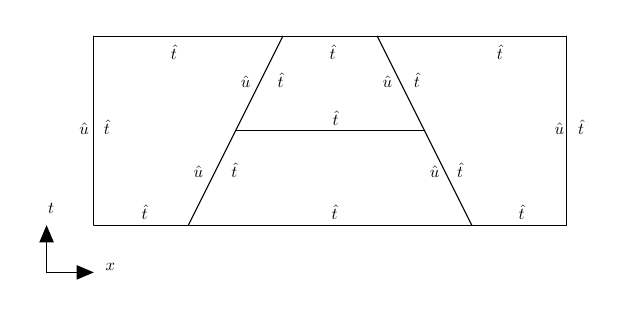
\begin{tikzpicture}[line cap=round,line join=round,>=triangle 45,x=2.0cm,y=2.0cm, scale=0.6, every node/.style={scale=0.6}]
\clip(-0.7,-0.6) rectangle (5.27,2.09);
\draw (0,2)-- (0,0);
\draw (0,0)-- (1,0);
\draw (1,0)-- (4,0);
\draw (4,0)-- (5,0);
\draw (5,0)-- (5,2);
\draw (5,2)-- (3,2);
\draw (3,2)-- (2,2);
\draw (2,2)-- (0,2);
\draw (1,0)-- (1.5,1);
\draw (1.5,1)-- (2,2);
\draw (1.5,1)-- (3.5,1);
\draw (3,2)-- (3.5,1);
\draw (3.5,1)-- (4,0);
\draw (-0.21,0.9) node[anchor=south west] {$\hat u$};
\draw (4.82,0.9) node[anchor=south west] {$\hat u$};
\draw (3.5,0.45) node[anchor=south west] {$\hat u$};
\draw (1.0,0.45) node[anchor=south west] {$\hat u$};
\draw (1.5,1.4) node[anchor=south west] {$\hat u$};
\draw (3.0,1.4) node[anchor=south west] {$\hat u$};
\draw (0.05,0.9) node[anchor=south west] {$\hat t$};
\draw (1.40,0.45) node[anchor=south west] {$\hat t$};
\draw (3.79,0.45) node[anchor=south west] {$\hat t$};
\draw (2.47,1.0) node[anchor=south west] {$\hat t$};
\draw (3.33,1.4) node[anchor=south west] {$\hat t$};
\draw (1.89,1.4) node[anchor=south west] {$\hat t$};
\draw (5.07,0.9) node[anchor=south west] {$\hat t$};
\draw (4.44,0.0) node[anchor=south west] {$\hat t$};
\draw (2.46,0.0) node[anchor=south west] {$\hat t$};
\draw (0.45,0.0) node[anchor=south west] {$\hat t$};
\draw (2.44,1.7) node[anchor=south west] {$\hat t$};
\draw (0.76,1.7) node[anchor=south west] {$\hat t$};
\draw (4.21,1.7) node[anchor=south west] {$\hat t$};
\draw [->] (-0.5,-0.5) -- (-0.5,0);
\draw [->] (-0.5,-0.5) -- (0,-0.5);
\draw (-0.54,0.29) node[anchor=north west] {$t$};
\draw (0.07,-0.35) node[anchor=north west] {$x$};
\end{tikzpicture}
\end{block}
\end{column}
\end{columns}
\end{frame}


% ------------------------------------------------------------
\begin{frame}[t]
\frametitle{Space-Time Convection-Diffusion}
\framesubtitle{Robust Norms}
% \vspace{-5ex}
\begin{columns}[t]
\begin{column}{0.5\textwidth}
\vspace{-3ex}

Bilinear form with group variables:
\[
b\LRp{\LRp{u,\hat u},v} = \LRp{u,A^*_h v}_{\LOmega} + \LRa{\uh, \jump{v}}_{\Gh}
\]
For conforming $v^*$ satisfying $A^* v^* = u$
\begin{align*}
&\norm{u}_{\LOmega}^2= b(u,v^*)
=\frac{b(u,v^*)}{\norm{v^*}_V} \norm{v^*}_V\\
&\quad\leq\sup_{v^*\neq0}\frac{|b(u,v^*)|}{\norm{v^*}}\norm{v^*}
=\norm{u}_E \norm{v^*}_V
\end{align*}
% If our test norm is bounded by $\norm{u}_{\LOmega}$,
% we can quarantee that 
% If $\norm{v^*}_V\lesssim\norm{u}_{L^2(\Omega_h)}$
% then $\Rightarrow\norm{u}_{L^2(\Omega_h)}\lesssim\norm{u}_E$.
Necessary robustness condition:
\begin{align*}
&\norm{v^*}_V\lesssim\norm{u}_{L^2(\Omega_h)}\\
&\quad\Rightarrow\norm{u}_{L^2(\Omega_h)}\lesssim\norm{u}_E
\end{align*}
\end{column}
\begin{column}{0.5\textwidth}
\vspace{-3ex}
\centering

Analytical Solution
\begin{align*}
u&=e^{-lt}(e^{\lambda_1(x-1)}-e^{\lambda2(x-1)})\\
\lambda_{1,2}&=\frac{-1\pm\sqrt{1-4l\epsilon}}{-2\epsilon}
\end{align*}
where $l=3, \quad\epsilon = 10^{-2}$
\vspace{-3ex}
\begin{figure}[t]
\centering
\includegraphics[width=\textwidth]{figs/SpaceTimeAnalyticalExact}
\end{figure}
\end{column}
\end{columns}
\end{frame}

% ------------------------------------------------------------
\begin{frame}[t]
\frametitle{Space-Time Convection-Diffusion}
\framesubtitle{Robust Norms}
A norm should be: bounded by $\norm{u}_{\LOmega}$, have good conditioning, not produce boundary layers in the optimal test function.
\vspace{-5ex}
\begin{columns}[t]
\begin{column}{0.5\textwidth}
\begin{figure}[t]
\centering
\includegraphics[width=\textwidth]{figs/SpaceTimeAnalyticalNorm0}
\end{figure}
\vspace{-5ex}
\small{
\begin{align*}
\norm{(v,\bftau)}^2&=
\norm{\Div\bftau-\tilde\bfbeta\cdot\Gradxt v}^2\\
&+\norm{\frac{1}{\epsilon}\bftau+\Grad v}^2
+\norm{v}^2
+\norm{\bftau}^2
\end{align*}
}
\end{column}
\begin{column}{0.5\textwidth}
\begin{figure}[t]
\centering
\includegraphics[width=\textwidth]{figs/SpaceTimeAnalyticalNorm4}
\end{figure}
\vspace{-5ex}
\small{
\begin{align*}
\norm{(v,\bftau)}^2&=
\norm{\Div\bftau-\tilde\bfbeta\cdot\Gradxt v}^2\\
&+\min\LRp{\frac{1}{h^2},\frac{1}{\epsilon}}\norm{\bftau}^2\\
&+\epsilon\norm{\Grad v}^2
+\norm{\bfbeta\cdot\Grad v}^2
+\norm{v}^2
\end{align*}
}
\end{column}
\end{columns}
\end{frame}

% ------------------------------------------------------------
\begin{frame}[t]
\frametitle{Space-Time Convection-Diffusion}
\framesubtitle{Ideal Optimal Shape Functions}
\vspace{-3ex}
\begin{columns}
\begin{column}{0.5\textwidth}
\begin{figure}[t]
\centering
Graph Norm
\includegraphics[width=0.8\textwidth]{OptimalTestFunctions/Graph_v}\\
\includegraphics[width=0.8\textwidth]{OptimalTestFunctions/Graph_tau}
\end{figure}
\end{column}
\begin{column}{0.5\textwidth}
\begin{figure}[t]
\centering
Robust Norm
\includegraphics[width=0.8\textwidth]{OptimalTestFunctions/Robust_v}\\
\includegraphics[width=0.8\textwidth]{OptimalTestFunctions/Robust_tau}
\end{figure}
\end{column}
\end{columns}
\end{frame}

% ------------------------------------------------------------
\begin{frame}[t]
\frametitle{Space-Time Convection-Diffusion}
\framesubtitle{Approximated ($p=3$) Optimal Shape Functions}
\vspace{-3ex}
\begin{columns}
\begin{column}{0.5\textwidth}
\begin{figure}[t]
\centering
Graph Norm
\includegraphics[width=0.8\textwidth]{OptimalTestFunctions/GraphApprox3_v}\\
\includegraphics[width=0.8\textwidth]{OptimalTestFunctions/GraphApprox3_tau}
\end{figure}
\end{column}
\begin{column}{0.5\textwidth}
\begin{figure}[t]
\centering
Robust Norm
\includegraphics[width=0.8\textwidth]{OptimalTestFunctions/RobustApprox3_v}\\
\includegraphics[width=0.8\textwidth]{OptimalTestFunctions/RobustApprox3_tau}
\end{figure}
\end{column}
\end{columns}
\end{frame}


\section{Camellia: DPG for the Masses}
\begin{frame}[fragile]
\frametitle{Camellia: DPG for the Masses}
\framesubtitle{Overview}  %% needed for proper positioning of the logo ...
\begin{block}{Design Goal}
Make DPG research and experimentation as simple as possible, while maintaining computational efficiency and scalability.
\end{block}
% \smallskip
Mature support for:
\begin{itemize}
  \item Rapid specification of DPG variational forms, inner products, etc.
  \item Distributed computation of stiffness matrix
  \item 1D - 3D geometries
  \item Curvilinear elements
  \item $h$- and $p$-refinements (anisotropic in $h$)
  \item Arbitrarily irregular meshes
  \item Modular refinement strategy interface
\end{itemize}
Experimental support for:
\begin{itemize}
  \item Space-time computations
  \item Iterative solvers (tested up to 32,768 cores)
\end{itemize}
\end{frame}

\begin{frame}[fragile]
\frametitle{Convection-Diffusion in Three Slides}
\framesubtitle{Building the Bilinear Form}  %% needed for proper positioning of the logo ...
\begin{columns}
\begin{column}{.6\textwidth}
\lstset{language=C++,
                basicstyle=\ttfamily\footnotesize,
                keywordstyle=\color{blue}\ttfamily,
                stringstyle=\color{red}\ttfamily,
                commentstyle=\color{green}\ttfamily,
                morecomment=[l][\color{magenta}]{\#}
}
\begin{lstlisting}
  VarFactory vf;
  //fields:
  VarPtr u = vf.fieldVar("u", L2);
  VarPtr sigma = vf.fieldVar("sigma", VECTOR_L2);
  
  // traces:
  VarPtr u_hat = vf.traceVar("u_hat");
  VarPtr t_n = vf.fluxVar("t_n");
  
  // test:
  VarPtr v = vf.testVar("v", HGRAD);
  VarPtr tau = vf.testVar("tau", HDIV);
  
  double eps = .01;
  FunctionPtr beta_x = Function::constant(1);
  FunctionPtr beta_y = Function::constant(2);
  FunctionPtr beta = Function::vectorize(beta_x, beta_y);
  
  BFPtr bf = Teuchos::rcp( new BF(vf) );
  
  bf->addTerm((1/eps) * sigma, tau);
  bf->addTerm(u, tau->div());
  bf->addTerm(-u_hat, tau->dot_normal());
  
  bf->addTerm(sigma - beta * u, v->grad());
  bf->addTerm(t_n, v);

  RHSPtr rhs = RHS::rhs();
\end{lstlisting}
% \begin{figure}
% \centering
% \includegraphics[width=0.9\textwidth]{figs/LightCamelliaDriver1}
% \end{figure}
\end{column}
\begin{column}{.4\textwidth}
\small
Find $u\in L^2(\Omega_h)$, $\bfsigma\in \bs L^2(\Omega_h)$, $\hat u\in H^{\frac{1}{2}}(\Gamma_h)$, $\hat t_n\in H^{-\frac{1}{2}}(\Gamma_h)$ \\
such that
\bigskip
\begin{align*}
&\frac{1}{\epsilon}\LRp{\bfsigma,\bftau}+\LRp{u,\Div\bftau}-\LRa{\hat u,\bftau\cdot\bfn}\\
&-\LRp{\bfbeta u-\bfsigma,\Grad v}+\LRa{\hat t_n,v}=\LRp{f,v}
\end{align*}
\bigskip
for all $v\in \HOneK$, $\bftau\in \HdivK$,
\bigskip
where $\epsilon=10^{-2}$, $\bfbeta=(1,2)^T$ and $f=0$.
\end{column}
\end{columns}
\end{frame}

\begin{frame}[fragile]
\frametitle{Convection-Diffusion in Three Slides}
\framesubtitle{Boundary Conditions and Mesh}  %% needed for proper positioning of the logo ...
\begin{columns}
\begin{column}{.7\textwidth}
\lstset{language=C++,
                basicstyle=\ttfamily\footnotesize,
                keywordstyle=\color{blue}\ttfamily,
                stringstyle=\color{red}\ttfamily,
                commentstyle=\color{green}\ttfamily,
                morecomment=[l][\color{magenta}]{\#}
}
\begin{lstlisting}
  int k = 2;
  int delta_k = 2;
  MeshPtr mesh = MeshFactory::quadMesh(bf, k+1, delta_k);

  BCPtr bc = BC::bc();
  
  SpatialFilterPtr y_equals_one = SpatialFilter::matchingY(1.0);
  SpatialFilterPtr y_equals_zero = SpatialFilter::matchingY(0);
  SpatialFilterPtr x_equals_one = SpatialFilter::matchingX(1.0);
  SpatialFilterPtr x_equals_zero = SpatialFilter::matchingX(0.0);
  
  FunctionPtr zero = Function::zero();
  FunctionPtr x = Function::xn(1);
  FunctionPtr y = Function::yn(1);
  bc->addDirichlet(t_n, y_equals_zero, -2 * (1-x));
  bc->addDirichlet(t_n, x_equals_zero, -1 * (1-y));
  bc->addDirichlet(u_hat, y_equals_one, zero);
  bc->addDirichlet(u_hat, x_equals_one, zero);
\end{lstlisting}
% \begin{figure}
% \centering
% \includegraphics[width=0.9\textwidth]{figs/LightCamelliaDriver2}
% \end{figure}
\end{column}
\begin{column}{.34\textwidth}
\small
Create a square mesh $[0,1]\times[0,1]$ with boundary conditions
\begin{itemize}
  \item $\hat t_n=2x-2$ on $y=0$
  \item $\hat t_n=x-1$ on $x=0$
  \item $\hat u=0$ on $y=1$
  \item $\hat u=0$ on $x=1$
\end{itemize}
Note
\begin{itemize}
  % \item Spatial Filters only act on boundary element edges
  \item Can subclass SpatialFilter to match any geometry
  \item Adding new mesh readers is straightforward
\end{itemize}
\end{column}
\end{columns}
\end{frame}

\begin{frame}[fragile]
\frametitle{Convection-Diffusion in Three Slides}
\framesubtitle{Test Norm, Solving, and Adaptivity}  %% needed for proper positioning of the logo ...
\begin{columns}
\begin{column}{.7\textwidth}
\lstset{language=C++,
                basicstyle=\ttfamily\footnotesize,
                keywordstyle=\color{blue}\ttfamily,
                stringstyle=\color{red}\ttfamily,
                commentstyle=\color{green}\ttfamily,
                morecomment=[l][\color{magenta}]{\#}
}
\begin{lstlisting}
  IPPtr ip = bf->graphNorm();

  SolutionPtr soln = Solution::solution(mesh, bc, rhs, ip);
  
  double threshold = 0.20;
  RefinementStrategy refStrategy(soln, threshold);
  
  int numRefs = 10;

  ostringstream refName;
  refName << "ConvectionDiffusion";
  HDF5Exporter exporter(mesh,refName.str());
  
  for (int refIndex=0; refIndex < numRefs; refIndex++) {
    soln->solve();
    
    double energyError = soln->energyErrorTotal();
    cout << "After " << refIndex << " refinements, energy error is " << energyError << endl;
    
    exporter.exportSolution(soln, vf, refIndex);
    
    if (refIndex != numRefs)
      refStrategy.refine();
  }
\end{lstlisting}
\end{column}
\begin{column}{.35\textwidth}
\small
\end{column}
\end{columns}
\end{frame}


\begin{frame}[fragile]
\frametitle{Convection-Diffusion in Three Slides}
\framesubtitle{Computed Solution}  %% needed for proper positioning of the logo ...
\begin{columns}[t]
\begin{column}{.5\textwidth}
\includegraphics[height=0.55\textheight]{Confusion/Tutorial/u_ref9.png}
\end{column}
\begin{column}{.5\textwidth}
\includegraphics[height=0.55\textheight]{Confusion/Tutorial/uhat_ref9.png}
\end{column}
\end{columns}
\end{frame}

%===============================================================================
% Poisson Iterative Solve Results
%===============================================================================

\newcommand{\plotscaling}{.8}
\newcommand{\plotscalingTwoUp}{.5}
\newcommand{\meshwidthindex}{4}
\newcommand{\iterationcountindex}{6}
\newcommand{\maxmyrows}{2000}
\newcommand{\PoissonOneDNthPoint}{5} %corresponds to the number of polynomial orders for which we ran the driver--here, 1,2,4,8,16
\newcommand{\PoissonTwoDNthPoint}{3} %corresponds to the number of polynomial orders for which we ran the driver--here, 1,2,4
\newcommand{\PoissonThreeDNthPoint}{2} %corresponds to the number of polynomial orders for which we ran the driver--here, 1,2
\newcommand{\PoissonOneDStride}{45}
\newcommand{\PoissonTwoDStride}{12}
\newcommand{\PoissonThreeDStride}{6}
\newcommand{\PoissonOneDSchwarzAlgebraicStart}{320} %for the k=16 results; technically, start is on 51, but 50 is the number we skip
\newcommand{\PoissonOneDSchwarzGeometricStart}{455}
\newcommand{\PoissonOneDGMGSchwarzAlgebraicStart}{50} %for the k=16 results; technically, start is on 51, but 50 is the number we skip
\newcommand{\PoissonOneDGMGSchwarzGeometricStart}{185}
\newcommand{\PoissonTwoDSchwarzAlgebraicStart}{87} %for the k=4 results; technically, start is on 88, but 87 is the number we skip
\newcommand{\PoissonTwoDSchwarzGeometricStart}{123}
\newcommand{\PoissonTwoDGMGSchwarzAlgebraicStart}{15} %for the k=4 results
\newcommand{\PoissonTwoDGMGSchwarzGeometricStart}{51}
\newcommand{\PoissonThreeDSchwarzAlgebraicStart}{32} %for the k=2 results
\newcommand{\PoissonThreeDSchwarzGeometricStart}{44}
\newcommand{\PoissonThreeDGMGSchwarzAlgebraicStart}{8} %for the k=2 results
\newcommand{\PoissonThreeDGMGSchwarzGeometricStart}{20}

\newcounter{algebraiccounter}
\newcounter{geometriccounter}

\newcounter{algebraiccounterk1}
\newcounter{geometriccounterk1}
\newcounter{algebraiccounterk2}
\newcounter{geometriccounterk2}

\begin{frame}
\frametitle{Towards a Robust Iterative Solver}
\framesubtitle{Poisson 1D, $p$-multigrid Preconditioners, $k=16$}  %% needed for proper positioning of the logo ...
\begin{figure}[ht]
  \centering
    \scalebox{\plotscaling}{
      \begin{tikzpicture}
      \begin{axis}[
          scaled ticks=false,
          tick label style={/pgf/number format/fixed},
          % title={Poisson 1D, $p$-multigrid Preconditioners, $k=16$}, 
          xlabel={Mesh Width (\# Elements)}, 
          ylabel={Iteration Count}, 
          grid=major,
          % legend entries={0 overlap (algebraic), 0 overlap (geometric), 1 overlap (algebraic), 1 overlap (geometric), 2 overlap (algebraic), 2 overlap (geometric)},
          legend pos=outer north east,
          xtick=data,
          xticklabels={2,,,,,64,128,256,512}
        ]
        \setcounter{algebraiccounter}{\PoissonOneDGMGSchwarzAlgebraicStart}
        \setcounter{geometriccounter}{\PoissonOneDGMGSchwarzGeometricStart}
        \addplot table [header=false, x index=\meshwidthindex, y index=\iterationcountindex, each nth point=\PoissonOneDNthPoint, skip first n=\value{algebraiccounter}, filter discard warning=false, unbounded coords=discard, skip coords between index={\PoissonOneDStride}{\maxmyrows}]{data/preconditioning/PoissonDriver1D_results_512_ranks_conforming.dat};
      \end{axis}
      \end{tikzpicture}
    }
  \label{fig:Poisson1Dk1GMG}
  \end{figure}
  Poisson 1D: number of CG iterations to reduce error by a factor of $10^{10}$ using $p$-multigrid preconditioners with Schwarz smoother with 0 overlap 
  for $k=16$.  The results for $k=1,2,4,$ and 8 are essentially identical.
\end{frame}

%===============================================================================
% Stokes Iterative Solve Results
%===============================================================================

\newcommand{\StokesTwoDNthPoint}{3} %corresponds to the number of polynomial orders for which we ran the driver--here, 1,2,4
\newcommand{\StokesThreeDNthPoint}{2} %corresponds to the number of polynomial orders for which we ran the driver--here, 1,2
\newcommand{\StokesTwoDStride}{12}
\newcommand{\StokesThreeDStride}{6}
\newcommand{\StokesTwoDSchwarzAlgebraicStart}{87} %for the k=4 results; technically, start is on 88, but 87 is the number we skip
\newcommand{\StokesTwoDSchwarzGeometricStart}{123}
\newcommand{\StokesTwoDGMGSchwarzAlgebraicStart}{15} %for the k=4 results
\newcommand{\StokesTwoDGMGSchwarzGeometricStart}{51}
\newcommand{\StokesThreeDSchwarzAlgebraicStart}{32} %for the k=2 results
\newcommand{\StokesThreeDSchwarzGeometricStart}{44}
\newcommand{\StokesThreeDGMGSchwarzAlgebraicStart}{8} %for the k=2 results
\newcommand{\StokesThreeDGMGSchwarzGeometricStart}{20}

\newcommand{\StokesThreeDSchwarzAlgebraicStartkOne}{31} %for the k=1 results
\newcommand{\StokesThreeDSchwarzGeometricStartkOne}{43}
\newcommand{\StokesThreeDGMGSchwarzAlgebraicStartkOne}{7} %for the k=1 results
\newcommand{\StokesThreeDGMGSchwarzGeometricStartkOne}{19}

\begin{frame}
\frametitle{Towards a Robust Iterative Solver}
\framesubtitle{Stokes 2D, $p$-multigrid Preconditioners, Schwarz algebraic overlap 0}  %% needed for proper positioning of the logo ...
  \begin{figure}[ht]
  \centering
    \scalebox{\plotscaling}{
      \begin{tikzpicture}
      \begin{axis}[
          % title={Stokes 2D, $p$-multigrid Preconditioners, Schwarz algebraic overlap 0}, 
          xlabel={Mesh Width (\# Elements)}, 
          ylabel={Iteration Count}, 
          grid=major,
          legend entries={$k=1$, $k=2$, $k=4$},
          legend pos=outer north east,
          xtick=data,
          xticklabels={2,,8,16,32,64},
          ytick={45,60,75,100,124}
        ]
        \addplot table [header=false, x index=\meshwidthindex, y index=\iterationcountindex, each nth point=3, skip first n=1, filter discard warning=false, unbounded coords=discard]{data/preconditioning/StokesDriver2D_results_nonconforming_GMG_algebraic_overlap0.dat};
        \addplot table [header=false, x index=\meshwidthindex, y index=\iterationcountindex, each nth point=3, skip first n=2, filter discard warning=false, unbounded coords=discard]{data/preconditioning/StokesDriver2D_results_nonconforming_GMG_algebraic_overlap0.dat};
        \addplot table [header=false, x index=\meshwidthindex, y index=\iterationcountindex, each nth point=3, skip first n=3, filter discard warning=false, unbounded coords=discard]{data/preconditioning/StokesDriver2D_results_nonconforming_GMG_algebraic_overlap0.dat};
      \end{axis}
      \end{tikzpicture}
    }
  \label{fig:Stokes2DExtras}
  \end{figure}
  \vspace{-5mm}
  Stokes 2D: number of CG iterations to reduce error by a factor of $10^{10}$ using $p$-multigrid, algebraic Schwarz smoother with 0 overlap.
\end{frame}


\begin{frame}
\frametitle{Towards a Robust Iterative Solver}
\framesubtitle{Stokes 3D, $p$-multigrid Preconditioners, $k=2$, Schwarz with Incomplete Cholesky}  %% needed for proper positioning of the logo ...
  \begin{figure}[ht]
  \centering
    \scalebox{\plotscaling}{
      \begin{tikzpicture}
      \begin{axis}[
          % title={Stokes 3D, $p$-multigrid Preconditioners, $k=2$, Schwarz with Incomplete Cholesky}, 
          xlabel={Mesh Width (\# Elements)}, 
          ylabel={Iteration Count}, 
          grid=major,
          % legend entries={0 overlap (algebraic), 1 overlap (algebraic)},
          legend pos=outer north east,
          xtick=data,
          xticklabels={2,4,8,16},
          ytick={46,91,136,167,197}
        ]
        \addplot table [header=false, x index=\meshwidthindex, y index=\iterationcountindex, each nth point=1, skip first n=1, filter discard warning=false, unbounded coords=discard]{data/preconditioning/StokesDriver3D_results_overlap0_IC_nonconforming.dat};
%       \addplot table [header=false, x index=\meshwidthindex, y index=\iterationcountindex, each nth point=1, skip first n=1, filter discard warning=false, unbounded coords=discard]{data/preconditioning/StokesDriver3D_results_overlap1_IC_nonconforming.dat};
      \end{axis}
      \end{tikzpicture}
    }
  \label{fig:Stokes3Dk2GMGIC}
  \end{figure}
  \vspace{-5mm}
  Stokes 3D: number of CG iterations to reduce error by a factor of $10^{10}$ using statically condensed system matrix with $p$-multigrid, algebraic Schwarz smoother, using Incomplete Cholesky factorization (fill ratio 5) for the Schwarz blocks.
\end{frame}


\section{Space-Time Compressible Navier-Stokes}
% ------------------------------------------------------------
\begin{frame}[t]
\frametitle{Space-Time Navier-Stokes}
\framesubtitle{First Order System}
Assuming Stokes hypothesis and ideal gas law:
\begin{align*}
  \frac{1}{\mu}\mathbb{D}-\LRp{\Grad\bfu+\LRp{\Grad\bfu}^T}+\frac{2}{3}\Div\bfu\bbI&=0\\
  \frac{Pr}{C_p\mu}\bfq+\Grad T&=0\\
  \Divxt\vecttwo{\rho\bfu}{\rho}&=f_c\\
  \Divxt\vecttwo{\rho\bfu\otimes\bfu+\rho RT\bbI-\mathbb{D}}{\rho\bfu}&=\bff_m\\
  \Divxt\vecttwo{\rho\bfu\LRp{C_v T+\frac{1}{2}\bfu\cdot\bfu}+\rho RT\bfu+\bfq-\bfu\cdot\mathbb{D}}{\rho\LRp{C_v T+\frac{1}{2}\bfu\cdot\bfu}}&=f_e\,,
\end{align*}
\end{frame}


% ------------------------------------------------------------
\begin{frame}[t]
\frametitle{Space-Time Navier-Stokes}
\framesubtitle{Compact Notation}
\begin{columns}[t]
\begin{column}{0.5\textwidth}
Conserved quantities
\vspace{-2ex}
\begin{align*}
C_c&:=\rho\\
\bfC_m&:=\rho\bfu\\
C_e&:=\rho(C_v T+\frac{1}{2}\bfu\cdot\bfu)\\
% C&:=\LRc{C_c\,,\, \bfC_m\,,\, C_e}\\
\end{align*}
\end{column} 
\begin{column}{0.5\textwidth}
Euler fluxes 
\vspace{-2ex}
\begin{align*}
\bfF_c&:=\rho\bfu\\
\bbF_m&:=\rho\bfu\otimes\bfu+\rho RT\bbI\\
\bfF_e&:=\rho\bfu\LRp{C_v T+\frac{1}{2}\bfu\cdot\bfu}+\rho RT\bfu\\
% F&:=\LRc{\bfF_c\,,\, \bbF_m\,,\, \bfF_e}\\
\end{align*}
\end{column} 
\end{columns}
\begin{columns}[t]
\begin{column}{0.3\textwidth}
Viscous fluxes 
\vspace{-2ex}
\begin{align*}
\bfK_c&:=\boldsymbol 0\\
\bbK_m&:=\bbD\\
\bfK_e&:=-\bfq+\bfu\cdot\bbD\\
% K&:=\LRc{\bfK_c\,,\, \bbK_m\,,\, \bfK_e}\\
\end{align*}
\end{column} 
\begin{column}{0.3\textwidth}
Viscous variables
\vspace{-2ex}
\begin{align*}
\bbM_{\bbD}&:=\frac{1}{\mu}\bbD\\
\bfM_{\bfq}&:=\frac{Pr}{C_p\mu}\bfq\\
% M&:=\LRc{\bbM_{\bbD}\,,\, \bfM_{\bfq}}\\
\end{align*}
\end{column} 
\begin{column}{0.3\textwidth}
Viscous relations
\vspace{-2ex}
\begin{align*}
\bfG_{\bbD}&:=2\bfu\\
G_{\bfq}&:=-T\\
% G&:=\LRc{\bfG_{\bbD}\,,\, G_{\bfq}}\\
\end{align*}
\end{column} 
\end{columns}
% \begin{align*}
% f&:=\LRc{f_c\,,\, \bff_m\,,\, f_e}\\
% \end{align*}
% and group variables
% \begin{align*}
% W&:=\LRc{\rho\,,\,\bfu\,,\,T}\\
% \hat W&:=\LRc{2\hat\bfu\,,\,-\hat T}\\
% \Sigma&:=\LRc{\bbD,\bfq}\\
% \hat t&:=\LRc{\hat t_e\,,\,\hat\bft_m,\,,\,\hat t_e}\\
% \Psi&:=\LRc{\bbS\,,\,\bftau}\\
% V&:=\LRc{v_c\,,\,\bfv_m,\,,\,v_e}\,.
% \end{align*}
\end{frame}


% ------------------------------------------------------------
\begin{frame}[t]
\frametitle{Space-Time Navier-Stokes}
\framesubtitle{Define Group Variables}
\begin{columns}[t]
\begin{column}{0.5\textwidth}
Group terms
\vspace{-2ex}
\begin{align*}
C&:=\LRc{C_c\,,\, \bfC_m\,,\, C_e}\\
F&:=\LRc{\bfF_c\,,\, \bbF_m\,,\, \bfF_e}\\
K&:=\LRc{\bfK_c\,,\, \bbK_m\,,\, \bfK_e}\\
M&:=\LRc{\bbM_{\bbD}\,,\, \bfM_{\bfq}}\\
G&:=\LRc{\bfG_{\bbD}\,,\, G_{\bfq}}\\
f&:=\LRc{f_c\,,\, \bff_m\,,\, f_e}\\
\end{align*}
\end{column}
\begin{column}{0.5\textwidth}
Group variables
\vspace{-2ex}
\begin{align*}
W&:=\LRc{\rho\,,\,\bfu\,,\,T}\\
\hat W&:=\LRc{2\hat\bfu\,,\,-\hat T}\\
\Sigma&:=\LRc{\bbD,\bfq}\\
\hat t&:=\LRc{\hat t_e\,,\,\hat\bft_m,\,,\,\hat t_e}\\
\Psi&:=\LRc{\bbS\,,\,\bftau}\\
V&:=\LRc{v_c\,,\,\bfv_m,\,,\,v_e}\,.
\end{align*}
\end{column}
\end{columns}
Navier-Stokes variational formulation is
\begin{align*}
\LRp{M,\Psi}+\LRp{G,\Div\Psi}-\LRa{\hat W,\Psi\cdot\bfn_x}&=0\\
-\LRp{\vecttwo{F-K}{C},\Gradxt V}+\LRa{\hat t,V}&=\LRp{f,V}\,.
\end{align*}
\end{frame}



% %    /$$$$$$                                                                            /$$ /$$       /$$          
% %   /$$__  $$                                                                          |__/| $$      | $$          
% %  | $$  \__/  /$$$$$$  /$$$$$$/$$$$   /$$$$$$   /$$$$$$   /$$$$$$   /$$$$$$$  /$$$$$$$ /$$| $$$$$$$ | $$  /$$$$$$ 
% %  | $$       /$$__  $$| $$_  $$_  $$ /$$__  $$ /$$__  $$ /$$__  $$ /$$_____/ /$$_____/| $$| $$__  $$| $$ /$$__  $$
% %  | $$      | $$  \ $$| $$ \ $$ \ $$| $$  \ $$| $$  \__/| $$$$$$$$|  $$$$$$ |  $$$$$$ | $$| $$  \ $$| $$| $$$$$$$$
% %  | $$    $$| $$  | $$| $$ | $$ | $$| $$  | $$| $$      | $$_____/ \____  $$ \____  $$| $$| $$  | $$| $$| $$_____/
% %  |  $$$$$$/|  $$$$$$/| $$ | $$ | $$| $$$$$$$/| $$      |  $$$$$$$ /$$$$$$$/ /$$$$$$$/| $$| $$$$$$$/| $$|  $$$$$$$
% %   \______/  \______/ |__/ |__/ |__/| $$____/ |__/       \_______/|_______/ |_______/ |__/|_______/ |__/ \_______/
% %                                    | $$                                                                          
% %                                    | $$                                                                          
% %                                    |__/    

% % ------------------------------------------------------------
% \begin{frame}[t]
% \frametitle{Compressible Navier-Stokes}
% \framesubtitle{Strong Form}  %% needed for proper positioning of the logo ...
% The compressible Navier-Stokes equations are
% \begin{align*}
% \frac{\partial}{\partial t}\svectthree{\rho}{\rho\bfu}{\rho e_0}
% +\Div\svectthree{\rho\bfu}{\rho\bfu\otimes\bfu+p\bfI-\mathbb{D}}{\rho\bfu e_0+\bfu p+\bfq-\bfu\cdot\mathbb{D}}
% %TODO: Possible error above. cfd-online seems to have T^T
% =\svectthree{f_c}{\bff_m}{f_e}\,,
% \end{align*}
% where
% \begin{equation*}
%   \mathbb{D}=2\mu\bfS^*=2\mu\LRs{\frac{1}{2}\LRp{\Grad\bfu+\LRp{\Grad\bfu}^T}-\frac{1}{3}\Div\bfu\bfI}\,,
% \end{equation*}
% \begin{equation*}
%   \bfq=-C_p\frac{\mu}{Pr}\Grad T\,,
% \end{equation*}
% and (assuming an ideal gas EOS)
% \[
% p=\rho R T\,.
% \]
% \end{frame}

% % ------------------------------------------------------------
% \begin{frame}[t]
% \frametitle{Compressible Navier-Stokes}
% \framesubtitle{First Order Space-Time Form}  %% needed for proper positioning of the logo ...
% Writing this in space-time in terms of $\rho$, $\bfu$, $T$, $\mathbb{D}$, and $\bfq$:
% \begin{align*}
%   \mathbb{D}-\mu\LRp{\Grad\bfu+\LRp{\Grad\bfu}^T}+\frac{2\mu}{3}\Div\bfu\bfI&=0\\
%   \bfq+C_p\frac{\mu}{Pr}\Grad T&=0\\
%   \Divxt\vecttwo{\rho\bfu}{\rho}&=f_c\\
%   \Divxt\vecttwo{\rho\bfu\otimes\bfu+\rho RT\bfI-\mathbb{D}}{\rho\bfu}&=\bff_m\\
%   \Divxt\vecttwo{\rho\bfu\LRp{C_v T+\frac{1}{2}\bfu\cdot\bfu}+\bfu\rho RT+\bfq-\bfu\cdot\mathbb{D}}{\rho\LRp{C_v T+\frac{1}{2}\bfu\cdot\bfu}}&=f_e\,.
% \end{align*}
% \end{frame}


% % ------------------------------------------------------------
% \begin{frame}[t]
% \frametitle{Compressible Navier-Stokes}
% \framesubtitle{DPG Formulation}  %% needed for proper positioning of the logo ...
% Multiplying by test functions and integrating by parts:
% % \scalebox{0.9}{
% {
% \small
% \begin{align*}
%   \LRp{\mathbb{D},\mathbb{S}}+\LRp{2\mu\bfu,\Div\mathbb{S}}-\LRp{\frac{2\mu}{3}\bfu,\Grad\trace{\mathbb{S}}}
%   -\LRa{2\mu\hat\bfu,\mathbb{S}\bfn_x}+\LRa{\frac{2\mu}{3}\hat\bfu,\mathbb{S}\bfn_x}&=0\\
%   \LRp{\bfq,\bftau}-\LRp{C_p\frac{\mu}{Pr}T,\Div\bftau}+\LRa{C_p\frac{\mu}{Pr}\hat T,\tau_n}&=0\\
%   -\LRp{\vecttwo{\rho\bfu}{\rho},\Gradxt v_c}+\LRa{\hat t_c,v_c}&=\LRp{f_c,v_c}\\
%   -\LRp{\vecttwo{\rho\bfu\otimes\bfu+\rho RT\bfI-\mathbb{D}}{\rho\bfu},\Gradxt\bfv_m}+\LRa{\hat\bft_m,\bfv_m}&=\LRp{\bff_m,\bfv_m}\\
%   -\LRp{\vecttwo{\rho\bfu\LRp{C_v T+\frac{1}{2}\bfu\cdot\bfu}+\bfu\rho RT+\bfq-\bfu\cdot\mathbb{D}}{\rho\LRp{C_v T+\frac{1}{2}\bfu\cdot\bfu}},\Gradxt v_e}
%   +\LRa{\hat t_e,v_e}&=\LRp{f_e,v_e}\,,
% \end{align*}
% }
% % }
% where $\hat u$ and $\hat T$ are spatial traces and $\hat t_c$, $\hat\bft_m$, and $\hat t_e$ are fluxes.
% \end{frame}


% % ------------------------------------------------------------
% \begin{frame}[t]
% \frametitle{Compressible Navier-Stokes}
% \framesubtitle{Flux and Trace Variables}  %% needed for proper positioning of the logo ...
% Spatial traces and fluxes are defined as follows:
% \begin{equation*}
% \begin{aligned}
% \hat\bfu&=\trace(\bfu)\\
% \hat T&=\trace(T)\\
% \hat t_c&=\trace\LRp{\rho\bfu}\cdot\bfn_x
% +\trace\LRp{\rho}n_t\\
% \hat\bft_m&=\trace\LRp{\rho\bfu\otimes\bfu+\rho RT\bfI-\mathbb{D}}\cdot\bfn_x
% +\trace\LRp{\rho\bfu} n_t\\
% \hat t_e&=\trace\LRp{\rho\bfu\LRp{C_v T+\frac{1}{2}\bfu\cdot\bfu}+\bfu\rho RT+\bfq-\bfu\cdot\mathbb{D}}\cdot\bfn_x\\
% &\quad+\trace\LRp{\rho\LRp{C_v T+\frac{1}{2}\bfu\cdot\bfu}}n_t\,.
% \end{aligned}
% \end{equation*}
% \begin{block}{Linearization}
% Fluxes, traces, and $\bfq$ are linear in the above bilinear form, but we need to linearize in $\rho$, $\bfu$, $T$, and $\mathbb{D}$ 
% (Jacobian and residual not shown here).
% \end{block}
% \end{frame}


% %TODO: Fix test norm
% % ------------------------------------------------------------
% \begin{frame}[t]
% \frametitle{Compressible Navier-Stokes}
% \framesubtitle{Test Norm}  %% needed for proper positioning of the logo ...
% \vspace{-3ex}
% {
% \small
% \begin{align*}
% &\norm{\Grad\bfv_m+\Grad v_e\otimes\tilde\bfu}^2+\norm{\Grad v_e}^2\\
% +&\left\|
% -\tilde\bfu\cdot\Grad v_c-\frac{\partial v_c}{\partial t}-\tilde\bfu\otimes\tilde\bfu:\Grad\bfv_m
% -R\tilde T\Div\bfv_m-\tilde\bfu\cdot\frac{\partial\bfv_m}{\partial t}\right.\\
% &\left.-C_v\tilde T\tilde\bfu\cdot\Grad v_e-\frac{1}{2}\tilde\bfu\cdot\tilde\bfu\tilde\bfu\cdot\Grad v_e
% -R\tilde T\tilde\bfu\Grad v_e
% -C_v\tilde T\frac{\partial v_e}{\partial t}-\frac{1}{2}\tilde\bfu\cdot\tilde\bfu\frac{\partial v_e}{\partial t}
% \right\|^2\\
% +&\left\|
% -\tilde\rho\Grad v_c
% -\tilde\rho\tilde\bfu\cdot\Grad\bfv_m-\tilde\rho\Grad\bfv_m\cdot\tilde\bfu
% -\tilde\rho\frac{\partial\bfv_m}{\partial t}
% -C_v\tilde\rho\tilde T\Grad v_e
% -\frac{1}{2}\tilde\rho\tilde\bfu\cdot\tilde\bfu\Grad v_e
% \right.\\
% &\left.
% -\frac{1}{2}\tilde\rho\tilde\bfu\cdot\Grad v_e\tilde\bfu
% -\frac{1}{2}\tilde\rho\Grad v_e\cdot\tilde\bfu\tilde\bfu
% -R\tilde\rho\tilde T\Grad v_e
% +\tilde{\mathbb{D}}\cdot\Grad v_e
% -\frac{1}{2}\tilde\rho\tilde\bfu\frac{\partial v_e}{\partial t}
% -\frac{1}{2}\tilde\rho\tilde\bfu\frac{\partial v_e}{\partial t}
% \right\|^2\\
% +&\left\|
% -R\tilde\rho\Div\bfv_m
% -C_v\tilde\rho\tilde\bfu\Grad v_e
% -R\tilde\rho\tilde\bfu\Grad v_e
% -C_v\tilde\rho\frac{\partial v_e}{\partial t}
% \right\|^2\\
% +&\|\frac{1}{\mu}\mathbb{S}\|^2
% +\norm{2\Div\mathbb{S}-\frac{2}{3}\Grad\trace{\mathbb{S}}}^2
% +\|\frac{Pr}{C_p\mu}\bftau\|^2
% +\norm{\Div\bftau}^2\\
% +&\norm{v_c}^2+\norm{\bfv_m}^2+\norm{v_e}^2
% \,.
% \end{align*}
% }
% \end{frame}


%    /$$$$$$                  /$$
%   /$$__  $$                | $$
%  | $$  \__/  /$$$$$$   /$$$$$$$
%  |  $$$$$$  /$$__  $$ /$$__  $$
%   \____  $$| $$  \ $$| $$  | $$
%   /$$  \ $$| $$  | $$| $$  | $$
%  |  $$$$$$/|  $$$$$$/|  $$$$$$$
%   \______/  \______/  \_______/
%                                
%                                
%        
% ------------------------------------------------------------
\begin{frame}[t]
\frametitle{Compressible Navier-Stokes}
\framesubtitle{Sod Shock Tube with $\mu=10^{-5}$}  %% needed for proper positioning of the logo ...
\foreach \n in {1,...,15}
{
\only<\n>
{
\vspace{-2ex}
\begin{figure}[ht]
\centering

\begin{subfigure}[c]{0.45\textwidth}
\centering
\includegraphics[height=0.7\textwidth]{Sod/MinNSDecoupled1e-5/den\n.pdf}
\end{subfigure}
\begin{subfigure}[c]{0.45\textwidth}
\centering
\includegraphics[height=0.7\textwidth]{Sod/MinNSDecoupled1e-5/vel\n.pdf}
\end{subfigure}
\begin{subfigure}[c]{0.45\textwidth}
\centering
\includegraphics[height=0.7\textwidth]{Sod/MinNSDecoupled1e-5/pres\n.pdf}
\end{subfigure}
\begin{subfigure}[c]{0.45\textwidth}
\centering
\includegraphics[width=1.0\textwidth]{Sod/MinNSDecoupled1e-5/mesh\n.png}
\end{subfigure}
\end{figure}
}
}
\end{frame}


%   /$$   /$$           /$$      
%  | $$$ | $$          | $$      
%  | $$$$| $$  /$$$$$$ | $$$$$$$ 
%  | $$ $$ $$ /$$__  $$| $$__  $$
%  | $$  $$$$| $$  \ $$| $$  \ $$
%  | $$\  $$$| $$  | $$| $$  | $$
%  | $$ \  $$|  $$$$$$/| $$  | $$
%  |__/  \__/ \______/ |__/  |__/
%                                
%                                
% 
% ------------------------------------------------------------
\begin{frame}[t]
\frametitle{Compressible Navier-Stokes}
\framesubtitle{Noh Implosion with $\mu=10^{-3}$}  %% needed for proper positioning of the logo ...
Infinitely strong shock propagation.
% \foreach \n in {9,...,9}
% {
% \only<\n>
% {
\vspace{4ex}
% \begin{figure}[ht]
% \centering

\begin{columns}[t] % contents are top vertically aligned
\begin{column}[T]{0.4\textwidth} % each column can also be its own environment
% \begin{subfigure}[c]{0.45\textwidth}
\centering
\includegraphics[height=1.0\textwidth]{Noh/MinNSDecoupled/den9.pdf}
\end{column}
% \end{subfigure}
\hspace{8ex}
\begin{column}[T]{0.55\textwidth} % each column can also be its own environment
% \begin{subfigure}[c]{0.4\textwidth}
\centering
\vspace{2ex}
\includegraphics[width=0.9\textwidth]{Noh/MinNSDecoupled/mesh9.png}\\
\centering
Sequence of 4 time slabs
\end{column}
\end{columns}
% \end{subfigure}
% \end{figure}
% }
% }

\end{frame}


\section{Related DPG Research}
\begin{frame}[t]
\frametitle{Related Research}
\framesubtitle{Past and Present Topics in DPG Research}  %% needed for proper positioning of the logo ...
\begin{itemize}
\item Multiphysics
\begin{itemize}
  \item Heat conduction (Poisson and Heat equation)
  \item Wave problems (Helmholtz and Maxwell)
  \item Linear elasticity and plate problems
  \item Convection-Diffusion, Stokes, incompressible Navier-Stokes, compressible Navier-Stokes, Euler
\end{itemize}
\item Natively nonlinear DPG
\item DPG for non-Hilbert $L^p$ spaces
\item Local conservation
\item Iterative solvers
\item Entropy scaling for physically meaningful test norms
\item General polyhedral elements
\end{itemize}
\end{frame}

% \section{Current and Future Work}
% \begin{frame}[t]
% \frametitle{Current and Future Work}
% \framesubtitle{~~}  %% needed for proper positioning of the logo ...
% \vspace{-3ex}
% Area A: Applicable Mathematics
% \begin{itemize}
%   \item Robustness analysis for space-time convection-diffusion
%   \item Explore positivity preserving techniques for compressible Navier-Stokes
% \end{itemize}
% \smallskip

% Area B: Scientific Computation
% \begin{itemize}
%   \item Support development of Camellia\footfullcite{CamelliaDPG}
%   \begin{itemize}
%     \item Development and verification of 2D space-time simulations.
%     \item Implement time slabs to decrease solve size
%     \item Contribute to auxiliary features
%   \end{itemize}
%   \item Run parallel simulations on HPC systems at TACC and ANL
%   % \item Investigate iterative solvers for DPG
% \end{itemize}
% \smallskip

% Area C: Modeling and Applications
% \begin{itemize}
%   \item Revisit Carter plate solve for higher Reynolds numbers
%   \item Incompressible Taylor-Green vortex problem
%   \item Incompressible vortex shedding problems
%   \item Possibly investigate compressible Sedov and Noh problems
% \end{itemize}
% \end{frame}


\begin{frame}[t]
\frametitle{Thank You!}
\framesubtitle{~~}
\vspace{-4ex}
\begin{figure}[ht]
\centering
\begin{subfigure}[c]{0.45\textwidth}
\centering
\animategraphics[autoplay,loop,width=0.99\textwidth]{1}{SpaceTimeCNS/Sod1e-5/den}{1}{15}
\end{subfigure}
\begin{subfigure}[c]{0.45\textwidth}
\centering
\animategraphics[autoplay,loop,width=0.99\textwidth]{1}{SpaceTimeCNS/Sod1e-5/vel}{1}{15}
\end{subfigure}
\begin{subfigure}[c]{0.45\textwidth}
\centering
\animategraphics[autoplay,loop,width=0.99\textwidth]{1}{SpaceTimeCNS/Sod1e-5/pres}{1}{15}
\end{subfigure}
\begin{subfigure}[c]{0.45\textwidth}
\centering
\animategraphics[autoplay,loop,width=0.99\textwidth]{1}{SpaceTimeCNS/Sod1e-5/mesh}{1}{15}
\end{subfigure}
\end{figure}
% \begin{center}
%   \animategraphics[autoplay,loop,width=0.6\textwidth]{1}{SpaceTimeCNS/Sod1e-5/den}{1}{15}
% \end{center}
\end{frame}


% \begin{frame}[t]
% \frametitle{Bibliography}
% \framesubtitle{~~}  %% needed for proper positioning of the logo ...
% {\oldfootnotesize
% \printbibliography
% }
% \end{frame}

\end{document}
